\documentclass[11pt,a4paper,twoside,openright]{book}

%\documentclass[11pt,a4paper]
%,twoside
%,draft
%{book} % Use the UniMelb Dissertation Template
\usepackage{style/uomthesis}
% User defined commands
\input{../SimpleResponsesChapter/user-defined}
\input{../SimpleResponsesChapter/glossary} % My glossary of terms
\makeglossary

% User defined commands
%\usepackage{pstricks}
\usepackage{appendix}

\usepackage{ctable}
 
%  \marginparwidth=3cm
% \addtolength{\oddsidemargin}{6mm}
%  \topmargin=0pt
%  \headsep=10pt
%  \voffset=-1.54cm
%  \hoffset=-1.54cm  %default hoffset is zero plus extra 1inch
%  \textwidth=16cm
%  \textheight=26cm
%  \renewcommand{\baselinestretch}{1.5}


\DeclareGraphicsRule{eps.gz}{eps}{.eps.bb}{zcat #1}
\newcommand{\figfont}[1]{\large{\textbf{\textsf{#1}}}}

\graphicspath{{./gfx/}{../figures/}}
\graphicspath{{../figures/}{/media/data/Work/thesis/GAChapter/gfx/}{/media/data/Work/thesis/GAChapter/archive/gfx/}{/media/data/Work/thesis-gaarticle/gfx/}{/media/data/Work/thesis-gaarticle/GApaper-submission-JCompNeuro/gfx/}}
%\usepackage[showlabels]{preview}
%\PreviewEnvironment[{*[][]{}}]{tabularx}
%\PreviewEnvironment[{*[][]{}}]{figure}
%\PreviewEnvironment[{*[][]{}}]{array}

\lfoot{\footnotesize\today\ at \thistime}

\begin{document}
%%%%%%%%%%%%%%%%%%%%%%%%%%%%%%%%%%%%%%%%%%%%%%%%%%%%%%

		% TOC, LOF, LOT
		{%
			\singlespacing%
                        \listoftodos
			\tableofcontents%
			%\listoffigures%
			% Do not include a list of tables if you have less
			% than 10 tables, as per SGS suggestion.
			%\listoftables%
                        \printglossary
		   \clearpage%
		}%

%{\today\ Hg changeset \input{.hg/tags.cache}}

\setcounter{chapter}{4}
\chapter[GAChapter]{GA optimsation of the CN stellate network}
\label{sec:GAChapter}


% \begin{synopsis}

%\end{synopsis}


%\PARstart{U}{se} the force Luke...

\section{Introduction}\label{sec:GA:intro}

Innovative methodologies, such as multi-unit recording
\citep{BrownKassEtAl:2004} and optical recording using
voltage-sensitive dyes
\citep{GrinvaldHildesheim:2004,YangDoiEtAl:2000}, are enabling
neuroscientists to monitor the simultaneous activity of networks of
neurons with a higher degree of spatial and temporal accuracy than has
been achieved previously at the network level. At the same time,
modeling {\BNN}s is becoming more
accessible and faster to run with modern computing power. (By
biophysically-based we mean models that include a description of
currents flowing through membrane ion channels, such as the
{\HH} model.)  To develop larger {\BNN}s, with complex network
behavior a number of interrelated issues need to be considered: (a)
what level of neuronal detail is required to achieve observed
phenomena in the network, (b) how do extrinsic and intrinsic noise
sources affect the model, and (c) how do we reliably constrain the
many free parameters in a model given limited experimental data.

\smallskip{} 

One set of approaches to constraining {\BNN}s, denoted as ``bottom-up'',
is to construct them using detailed knowledge of specific neurons and
their membrane current properties. These bottom-up approaches to
neural modeling have been quite successful at representing single cell
models. They are, however, insufficiently sophisticated when it comes
to constraining the free parameters in small networks of neurons
\citep{GrillnerMarkramEtAl:2005,KochSegev:1998}, generally relying on
hand-tuning parameters. In contrast, the ``top-down'' approach to
constraining neural network models uses the output of the network
activity to infer the underlying model parameters. Such networks were
originally developed to be abstract feature detectors
\citep{Malsberg:1973} or simple nerve field projections
\citep{Amari:1980} based on general principles of neural processing.
Optimization and training algorithms for top-down network constraint
are highly efficient and generally involve a gradient-decent search
with a training method called back-propagation, where the output error
is calculated back through the network
\citep{RumelhartHintonEtAl:1986a}. These algorithms are not applicable
to {\BNN}s because the input/output relationships of Hodgkin-Huxley-type
models are not analytical, making them unsuitable for error
back-propagation.

\smallskip{} 

The particular challenges of constraining network parameters in {\BNN}s
or ensembles of spiking neural networks, which have been discussed
previously \citep{EggertHemmen:2001,Brette:2007} focus on the
analytical methods characterizing the spike output~\citep{Victor:2005,KostalLanskyEtAl:2007,BrownKassEtAl:2004}. Inferring
the connectivity within a network requires a cost analysis of the
spiking output.  This has progressed from ensemble feature-based
methods~\citep{SameshimaBaccala:1999,DahlhausEichlerEtAl:1997,TheunissenSenEtAl:2000},
information theoretical approaches using maximum likelihood
\citep{YamadaMatsumotoEtAl:1996,Chichilnisky:2001,OkatanWilsonEtAl:2005,PaninskiPillowEtAl:2004},
evolutionary algorithm methods~\citep{TakahamaSakai:2005,Yao:1999},
and other non-linear approaches~\citep{Eblen-ZajjurSalasEtAl:1999}.
However, most of these efforts have been restricted to single neuron
models or networks of integrate-and-fire neural models rather than
{\BNN}s.

\smallskip{} 

Genetic Algorithms (GAs) belong to a class of optimization algorithms
that mimic the process of evolution through natural selection. The
primary strength of {\GA}s relative to other optimization techniques,
such as gradient-descent, is that {\GA}s can avoid getting caught in
local minima \citep{Goldberg:1989,Whitley:1995}. Since
\citet{Holland:1975} first used {\GA}s to evolve the connectivity and
synaptic weights of artificial neural networks, some other hybrid
methods have been proposed \citep{Yao:1999,Whitley:1995}. Existing
examples of biophysically-based neural models that have been
constrained using {\GA}s are limited to single and multi-compartmental
single cell models \citep{KerenPeledEtAl:2005,VanierBower:1999,VanDeEtAl:2008} or small
microcircuits \citep{TaylorEnoka:2004}.  They are generally regarded
as an effective method in automated
parameter-searches. \citet{KerenPeledEtAl:2005} used intracellular
recordings from a cortical pyramidal cell to constrain the membrane
conductances of a multi-compartmental model.  The synaptic input noise
was filtered out, enabling the model data to be fit to experimental
recordings. \citet{TaylorEnoka:2004} used a microcircuit of spinal
motor units that was trained using feature-based analysis of the
output to fit the membrane and synaptic parameters.  Ongoing work in
{\BNN} modeling \citep{VanierBower:1999,VanDeEtAl:2008} is making headway
in removing the hand-tuning of parameters, but the application to
medium and large-scale networks may require more techniques from the
top-down methods in cost analysis and optimization algorithms.

\smallskip{} 

This section of the thesis investigates the application of {\GA}s in
constraining synaptic parameters in a topographically-ordered {\BNN},
using the example of a network in the auditory brainstem. The design
of the {\GA}, outlined in the Methods, includes the specification of a
cost function that measures how well the model network reproduces the
target data. We assess three alternate cost functions derived, in
different ways, from the output of neural responses in the
network. Each cost function is based on measures of (1) spike timing,
(2) instantaneous firing rate, or (3) average intracellular
voltage. Surrogate data from a randomly generated network model served
as our target and the ability of the algorithms to find the known
neural parameters was assessed. To analyze the robustness of the cost
functions to synaptic noise and the effects of trial-to-trial
variability we incorporated these effects into the model.

\subsection{Stellate Microcircuit of the Cochlear
  Nucleus}\label{sec:GA:stell-micr-cochl}

The network used as the basis for optimising {\BNN}s lies in the cochlear
nucleus (CN, Figure~\ref{fig:GA:CNdiagram}), which is the gateway
between the peripheral auditory system and the central nervous system,
with six distinct pathways to higher auditory nuclei
\citep{CantBenson:2003}. The principle neurons in the circuit are the
T-stellate (TS) cells, in the \VCN,
(Figure~\ref{fig:GA:CNdiagram}), which project to the inferior
colliculus.  They provide a robust spectral representation of sound
and are implicated in forming part of the main `what' pathway for
auditory information \citep{YoungOertel:2004}. Experimental evidence
indicates that synaptic inputs from inhibitory interneurons play a
critical role in modulating the input-output response properties of TS
neurons
\citep{FerragamoGoldingEtAl:1998,NeedhamPaolini:2006,PaoliniClareyEtAl:2005}.
The neurons TS, together with their inhibitory interneurons and
afferent inputs, form a microcircuit, which we have taken as our
example network.


 \begin{figure}[pt!]
\centering
   \resizebox{5in}{!}{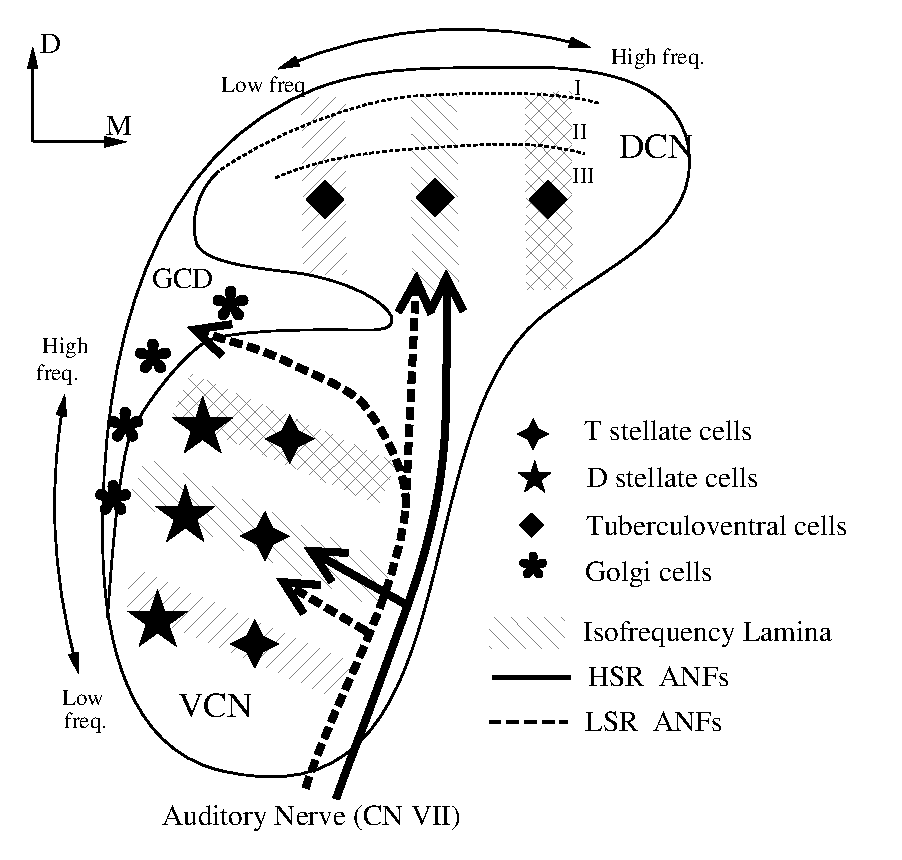
\includegraphics{CNConnections3}}
   \caption{Diagram of the mammalian cochlear nucleus. {ANF}s
     sensitive to particular frequencies project to the cochlear
     nucleus (CN) in a tono-topically organized fashion and bifurcate
     to innervate both the {VCN} and {DCN}. The {CN} comprises
     two main divisions, ventral and dorsal CN, plus an outer layer of
     small cells known as the granule cell domain (GCD). Type I
     {ANF}s are characterized into two groups based on their
     spontaneous rate: high (HSR, solid line) and low (LSR, dashed
     line). Only LSR and smaller type II {ANF}s project to the {GCD}.
     Golgi cells in the {GCD} are the only known source of {GABA}ergic
     cells within the VCN, and it is presumed that they synapse with
     TS and DS cells \citep{FerragamoGoldingEtAl:1998}. Glycinergic
     D-stellate cells (DS) project to wide areas of the VCN, DCN,
     and contralateral {CN}. DS cells are broadly tuned and respond
     best at the onset of a tone, with a small number of precisely
     timed spikes, and respond strongly to broad-band noise.  In the
     deep layer of the DCN, tuberculo-ventral (TV) cells provide
     a narrow-band on-frequency source of glycinergic inhibition to
     the VCN. These neurons respond poorly to clicks and
     broad-band noise, due to wide-band inhibition from DS cells
     \citep{SpirouDavisEtAl:1999}.}
\label{fig:GA:CNdiagram}
 \end{figure}
% \clearpage


\begin{figure}[t!]
\centering
\figfont{A}\hspace{3in}\\
\resizebox{3in}{!}{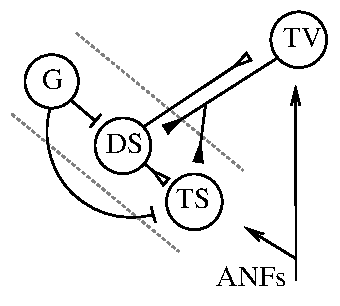
\includegraphics{SimpleCircuit3}}\\
\figfont{B}\hspace{3in}\\
\resizebox{3in}{!}{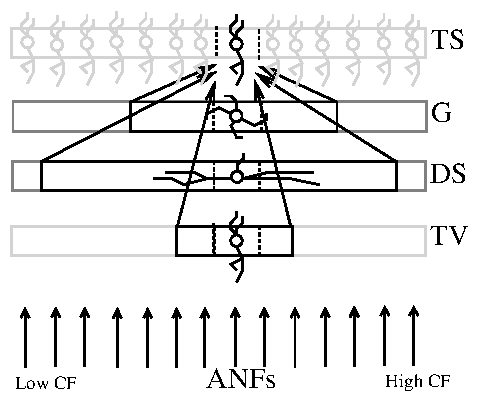
\includegraphics{NetworkProjections3}}\\
\caption{(A) Stellate microcircuit showing synaptic interaction within
  one iso-frequency lamina of the ventral {CN} (dotted lines) and TV
  cells of the dorsal CN\@. Excitatory synapses from {ANF}s (arrows)
  are modulated within the network by glycinergic (triangle) and
  GABAergic (T) inputs. (B)~ANFs are ordered into a wide range of
  frequency channels that are mapped to the ventral {CN} and dorsal
  CN in an orderly, tono-topic fashion. Topographic organization of
  lateral connections in the {CN} stellate network shows the range of
  inputs to TS cells from Golgi, DS and TV cells. Dendritic
  morphologies of cells characterize the range of {ANF} inputs and
  hence determine their frequency response. {ANF} input to TS and TV
  cells are restricted to one iso-frequency lamina, whereas DS
  dendrites span 1/3 of the ventral CN\@. DS cells' axonal plexus
  typically covers 1/3 of the ventral {CN} and one half of the dorsal
  CN, giving them a strong influence throughout the {CN}
  \citep{ArnottWallaceEtAl:2004}.}\label{fig:GA:MicroCN}
\end{figure}

\smallskip{} 

The tonotopic organization of the auditory pathway (i.e.\ the
continuous mapping of sound frequency to place of resonance in the
cochlea) is transferred to the {\CN} through the population of auditory
nerve fibers (ANFs)
\citep{Lorente:1981}. Figure~\ref{fig:GA:CNdiagram} shows that ANFs
enter the brainstem ventrally and bifurcate, so that each fiber sends
axonal collaterals to the ventral and dorsal sections of the cochlear
nucleus, to organized iso-frequency lamina. {\ANF}s are categorized into
high spontaneous rate (HSR, Figure~\ref{fig:GA:CNdiagram} solid line)
and low spontaneous rate (LSR, Fiqure~\ref{fig:GA:CNdiagram} dashed
line) fibers. LSR fibers have a higher threshold than HSR fibers and
do not saturate in response to loud sounds.

\smallskip{} 

The connectivity of the cell types involved in the stellate
microcircuit is shown in Figure~\ref{fig:GA:MicroCN}. Fast,
glycinergic inhibition from Tuberculoventral (TV) cells and D-stellate
cells (DS, Figure~\ref{fig:GA:CNdiagram}) is involved in modulating
the firing rate and spike interval variability in TS cells
\citep{FerragamoGoldingEtAl:1998,WickesbergOertel:1993}. TV cells in
the deep layer of the dorsal CN, provide a delayed narrowband
inhibition to TS and DS cells in the \VCN\@.  The dendrites of
DS cells cover 1/3~of the cross-frequency axis in the \CN, contributing
to this cell's wide frequency response. In turn this cell is
responsible for altering the frequency responses in TS and TV cells
\citep{SpirouDavisEtAl:1999}. DS cells are coincidence detectors and
have a precisely timed onset response that affects the temporal
properties of TS cells
\citep{PaoliniClareyEtAl:2005,RhodeGreenberg:1994a} and completely
inhibit TV cell responses to loud clicks
\citep{SpirouDavisEtAl:1999}. GABAergic inhibition from Golgi cells
(Figure~\ref{fig:GA:CNdiagram}) modulates the level of excitation
necessary to reach threshold for all {\CN} cells
\citep{CasparyBackoffEtAl:1994,FerragamoGoldingEtAl:1998}. Feedback
circuits from the olivary complex to the ventral {\CN} are also known to
use {GABA} as a neurotransmitter \citep{SaintMorestEtAl:1989}, however
this is not included in the model.

\smallskip{} 

\section{Methods}

\subsection{Genetic Algorithm Implementation }

For a model constraining problem, genetic algorithms work by searching
across successive generations of models for the model that is
``fittest'' in the sense that it best reproduces some user supplied
data. Each generation of models is obtained from the previous one by
using fitness-based selection criteria to create new models from
existing members of the population. In this process a model is
represented by a genome, which is the result of mapping the model
parameters into binary strings and concatenating them together. Each
population of genomes is evaluated for fitness using a carefully
tailored cost-function, better fitness increases the probability that
a genome will contribute to the next population.  The basic principles
of genetic reproduction, viz.\ crossover operation and mutation, are
used to generate new genomes from selected existing genomes. A
crossover operation breaks two genomes at a random location and swaps
their tail portions to create two new genomes. A mutation is a random
bit reversal in a genome. Crossover operations ensure that there is
adequate mixing of the best performing genomes in the population and
mutations are introduced to ensure diversity. The best members of the
population are usually copied (cloned) in the new population.

\smallskip{} 

In this work, all {\GA} simulations ran with 100~genomes in each
population and evolved for 200~generations. From each population, a
new population was created by cloning the five best genomes and
performing the following procedure for the remaining 95~genomes.
Candidate genomes for crossover were randomly selected based on their
fitness, using the roulette-wheel selection probability function,
where each score was linearly scaled so that the probability of
selection, $P_i$, is:
\begin{equation} \label{eq:GA:1} 
P_{i} =1 - \frac{g_{i} }{G}
\end{equation}
\noindent where $g_i$ is the genome's cost-function score, and $G$ is
the sum of all genome scores in the current population (note that the
sign in front of $g_i$ is negative here, instead of the conventional
positive, because we use cost-functions corresponding to an error
term, so that smaller values of $g_i$ imply greater
fitness). Following selection of a genome, crossover occurred with a
strictly different selected genome, with probability 0.95.
Alternatively the selected genome was cloned, with probability 0.05.
For the group of 95~genomes, a random bit mutation was implemented
with probability 0.01. The best performing genome string at the end of
the 200th generation was declared the winner.

\smallskip{} 

Parameters that were optimized were the synaptic weights, number of
synaptic connections per neuron and a parameter describing the spatial
variance of connections (details are given in the
section~\ref{sec:GA:connectivity} Connectivity). The genome encoding
scheme, shown in Table~\ref{tab:GA:Genome}, describes the number of bits
used for each parameter and the range of values that each parameter
could take.  For example, the first parameter in Table~\ref{tab:GA:Genome},
$w_{{\rm ANF}\to{\rm TS}}$ models the strength of synapses from {\ANF} to
TS cells. It was encoded over the range 0.0-0.0051 $\mu$S using 8~bits
by assigning 0b00000000~to 0.0~and 0b11111111~to 0.0051, and linearly
interpolating all values within the range. This procedure was used for
all parameters where the unit step was either 0.0001 $\mu$S for weight
parameters or 1 (synaptic connection or frequency channel) for all
others. The number of bits representing each parameter was chosen so
that the maximum value lay outside of known physiological
values. Genomes were formed by concatenating all these parameter bit
strings in the order given in Table~\ref{tab:GA:Genome}.

\smallskip{}

To test the application of {\GA}s for optimizing parameters of a {\BNN}, a
network with a known set of parameters was created, this is referred
to as the target network.  This allowed us to assess the {\GA} by how
well the algorithm was able to recover the target parameters. The
target parameters were randomly selected from within the physiological
range of values and given in Table~\ref{tab:GA:Genome}.  Target data
were generated from the target network and used as training data for
the {\GA} by incorporating them in an error-based cost function.  A
notch-noise stimulus (described under Stimulus Generation) was chosen
to present to the network as it produced a spectrally rich response
that was spread over the whole frequency range of the target network.
Figure 3A shows a spike raster plot for all TS cells to a presentation
of the notch noise stimulus. The vertical axis is arranged according
to the frequency to which the neuron is most sensitive (the center
frequency). There is a clear reduction in the firing rate
corresponding to the stop band in the
notch-noise. Figure~\ref{fig:GA:Costfunctions}B illustrates response
to 250~repetitions for a single TS cell in the center of the network,
at the rising edge of the notch (arrow in
Figure~\ref{fig:GA:Costfunctions}A).

%\begin{center}
\begin{table}[tp]
 \centering
 \caption{Network Parameter-to-Genome Encoding Scheme}\label{tab:GA:Genome}
 \begin{tabularx}{0.7\textwidth}{lccccc}   \toprule
  &           Parameter           & Binary Bits & \multicolumn{2}{c}{Range} & Target Value \\\midrule
1  & $w_{{\rm ANF}\to {\rm TS}} $  &  8  & 0.0 &  0.0051   & 0.00270 \\ %\hline
2  & $n_{{\rm LSR}\to {\rm TS}} $  &  5  &  0  &    31     & 7 \\ %\hline
3  & $n_{{\rm HSR}\to {\rm TS}} $  &  5  &  0  &    31     & 22 \\ %\hline
4  & $w_{{\rm ANF}\to {\rm DS}} $  &  8  & 0.0 &  0.0051   & 0.00178 \\ %\hline
5  & $n_{{\rm ANF}\to {\rm DS}} $  &  6  &  0  &    63     & 27 \\ %\hline
6  & $n_{{\rm HSR}\to {\rm DS}} $  &  6  &  0  &    63     & 59 \\ %\hline
7  & $w_{{\rm ANF}\to {\rm TV}} $  &  8  & 0.0 &  0.0051   & 0.00091 \\ %\hline
8  & $n_{{\rm LSR}\to {\rm TV}} $  &  5  &  0  &    31     & 13 \\ %\hline
9  & $n_{{\rm HSR}\to {\rm TV}} $  &  5  &  0  &    31     & 16 \\ %\hline
10 & $w_{{\rm LSR}\to {\rm GLG}} $ &  8  & 0.0 &  0.0051   & 0.00150 \\   %\hline
11 & $n_{{\rm LSR}\to {\rm GLG}} $ &  5  &  0  &    31     & 16 \\   %\hline
12 &  $w_{{\rm DS}\to {\rm TS}} $  &  8  & 0.0 &  0.0051   & 0.00028 \\ %\hline
13 &  $n_{{\rm DS}\to {\rm TS}} $  &  5  &  0  &    31     & 14 \\ %\hline
14 &  $s_{{\rm DS}\to {\rm TS}} $  &  6  &  0  &    63     & 15 \\   %\hline
15 &  $w_{{\rm TV}\to {\rm TS}} $  &  8  & 0.0 &  0.0051   & 0.00040 \\ %\hline
16 &  $n_{{\rm TV}\to {\rm TS}} $  &  5  &  0  &    31     & 12 \\ %\hline
17 &  $s_{{\rm TV}\to {\rm TS}} $  &  5  &  0  &    31     & 3 \\   %\hline
18 & $w_{{\rm GLG}\to {\rm TS}} $  &  8  & 0.0 &  0.0051   & 0.00022 \\ %\hline
19 & $n_{{\rm GLG}\to {\rm TS}} $  &  5  &  0  &    31     & 7 \\ %\hline
20 & $s_{{\rm GLG}\to {\rm TS}} $  &  5  &  0  &    31     & 3 \\   %\hline
21 &  $w_{{\rm DS}\to {\rm TV}} $  &  8  & 0.0 &  0.0051   & 0.00042 \\ %\hline
22 &  $n_{{\rm DS}\to {\rm TV}} $  &  6  &  0  &    63     & 18 \\ %\hline
23 &  $s_{{\rm DS}\to {\rm TV}} $  &  6  &  0  &    63     & 8 \\   %\hline
24 &  $w_{{\rm TV}\to {\rm DS}} $  &  8  & 0.0 &  0.0051   & 0.00016 \\ %\hline
25 &  $n_{{\rm TV}\to {\rm DS}} $  &  6  &  0  &    63     & 7   \\ %\hline
26 &  $s_{{\rm TV}\to {\rm DS}} $  &  6  &  0  &    63     & 3 \\   %\hline
27 &  $o_{{\rm DS}\to {\rm TV}} $  &  5  &  0  &    31     & 3 \\ %\hline
28 & $w_{{\rm GLG}\to {\rm DS}} $  &  8  & 0.0 &  0.0051   & 0.00246 \\   %\hline
29 & $n_{{\rm GLG}\to {\rm DS}} $  &  5  &  0  &    31     & 7 \\ %\hline
30 & $s_{{\rm GLG}\to {\rm DS}} $ &  5  &  0  &    31     & 5 \\[0.5ex] \bottomrule
\end{tabularx}\\
\vspace{0.5ex} 
\footnotesize{Units of weights are $\mu$S. $n$ and $s$
  parameters are unitless integers. The resolution of weight
  parameters were set to 0.0001 $\mu$S and other parameters to 1.}
\end{table}
%\end{center}




\subsection{Cost functions}\label{sec:GA:cost-functions}

At the core of a {\GA} optimization is a cost function, which is given,
here, by an error measure of some observable output of a trial network
against the output of the target network. In this work, the total cost
function score is calculated using the output of all cells in the
network.  Three different cost functions were investigated that were
based on experimental observables: spike times, instantaneous firing
rates, and intracellular voltages.


\begin{figure}[pt!]
  \begin{center}
%\setlength{\unitlength}{1pt}
    \resizebox{2.5in}{!}{%
\begin{picture}(206,108)(0,0)
  \put(0,0){\includegraphics[bb=98 523 304 631,clip]{Figure3}}
  \put(25,48){\thicklines\vector(1,0){10}}
  \end{picture}}%
    \resizebox{2.5in}{!}{\includegraphics[bb=98 411 304 523,clip]{Figure3}}\\
    \vspace{0.1in}\resizebox{5in}{!}{\includegraphics[bb=98 173 504 411,clip]{Figure3}}
\end{center}
\caption{Cost function measures derived from the output of the CN
  stellate network. (A) Dot raster of TS cell spikes only during a
  presentation of the notch noise stimulus. A rough trace shows the
  relative location of the 30-dB notch in a broadband spectrum from
  0.2~to 30 kHz. Frequency scale is determined by the Greenwood
  function for the cat \citep{Greenwood:1990}. (B) The reference spikes
  for a TS cell in the middle of the `target' network (CF 3.45kHz)
  from 250 repetitions of the stimulus are shown. This cell is placed
  at the edge of the spectral notch (arrow in A.). (C) PSTH response
  of the same TS cell used in B (bin width 0.25~ms, reps. 250). Note
  the regularly-spaced peaks at the start of the stimulus due to the
  TS cells' chopper response characteristics. Irregular peaks
  throughout the stimulus are due to temporal features of the notch
  noise captured by the auditory filter at this frequency. (D) PSTH of
  the same cell as in C using only 25 repetitions. The IFR cost
  function normalizes the reference PSTHs and calculates a mean
  squared error between reference and test {PSTH}s for every cell in the
  network. (E) Average intracellular voltage, smoothed from 250
  repetitions, for the same TS cell. There is some similarity with the
  PSTH in C, particularly the location of the peaks but contains
  subthreshold effects. (F) Average intracellular voltage using 25
  repetitions is more variable than E since single action potentials
  can distort the trace.}
\label{fig:GA:Costfunctions}
\end{figure}
\clearpage

\subsubsection{Spike Timing Cost Function}\label{sec:GA:spike-timing-cost-fn}


Spike times give accurate temporal information but are limited by a
focus on individual stimulus presentations, which may contain various
sources of noise and trial-to-trial variability. The metric we used
for comparing trial and target spike trains applied a cost based on
relative timing of spikes, for a review see \citet{Victor:2005}.

\smallskip{}

The spike timing (ST) cost function was defined as:
\begin{equation} \label{eq:GA:2} 
\Psi _{{\rm ST}} = \frac{1}{N_{{\rm ST}}
  } \sum _{i=1}^{M}\sum _{j=1}^{R}\mathop{\min}\limits_{k}
  \left(D\left(x_{ij} ,x_{ik}^{*} \right)\right)
\end{equation}
\noindent where $N_{{\rm ST}} =R\times M$ is a normalization factor,
$M=240$~is the number of neurons in the network, $R=25$ is the total
number of stimulus repetitions, $x_{ij}$ is the vector containing the
spike times of the trial network for stimulus repetition $j$ produced
by neuron $i$, and $x_{ik}^{*}$ is the vector containing the spike
times of the target network for the stimulus repetition $k$ produced
by neuron $i$.  The units for $\Psi_{{\rm ST}}$ are ms per cell per
spike train for 60~ms duration spike trains but will be milliseconds
for the remainder of the study. $D(x_{ij} ,x_{ik}^{*})$ is the
difference measure between trial and target network spike trains as
found by dynamic programming.  Dynamic programming is a method for
analyzing sequential processes \citep{Denardo:1982} and was applied to
find the minimum distance between two spike trains, as illustrated in

\begin{figure}[t!]
 \resizebox{3in}{!}{gfx/DynamicSpikeMetric_v2.TpX}
 \caption{Spike timing cost function measure computed using a dynamic
   programming algorithm. A minimum distance matrix between the
   \textit{target} set of spike times and a \textit{trial} set of
   spike times (from the same cell in the network, $i$, is traversed
   to find the minimum cumulative path of timing errors. Arrows
   indicate the possible combinations of spike time errors. For every
   cell, each repetition in the trial set, $j$, is compared against 25
   repetitions, $k$, in the training data to find the best fit and to
   minimize penalties for missing or additional spikes.}
\label{fig:GA:DynSpikeMetric}
\end{figure}

\smallskip{}

Figure~\ref{fig:GA:DynSpikeMetric}.  In this process, a trial spike
train, $x_{ij}$, was mapped onto a target spike train, $x_{ik}^{*}$,
by a process of realignment, without specifically considering
insertion or deletion of spikes. Insertion and deletion of spikes
require additional penalties and have been used in single spike trains
\citep{VictorGoldbergEtAl:2007,Aronov:2003}.  The cost associated with
a spike in the trial network and a spike in the target network was
measured as the time difference between the spikes. The spikes to
select for comparison were chosen such that the overall cost was
minimized.

\smallskip{}

We chose the minimum value of $D(x_{ij} ,x_{ik}^{*} )$ over 25~target
network spike-time vectors, $x_{ik}^{*}$, $k=1,\dots,25$, to reduce
the effect of output randomness, it was limited to 25~vectors to
obtain a reasonable computational load.  In the case where a trial
network produces no output spikes, $D(x_{ij} ,x_{ik}^{*})$ is the sum
of the target spike times, no target neurons produced empty spike
trains.

\smallskip{}

To illustrate the behavior of this cost function in the ideal case,
where {\ANF} inputs to the trial network are the identical those used in
the 25~repetitions of the target data and the target network
parameters are used, the value of $\Psi_{{\rm ST}}$ is zero. The
maximum value of $\Psi_{{\rm ST}}$ observed in this study was
approximately 360~ms.  For an example trial network that produces the
correct number of spikes for each neuron but with an average spike
timing error of 1~ms, given that the average number of spikes per
train is 9, the cost function would be $\Psi_{{\rm ST}}=9$~ms per
spike train.



\subsubsection{Instantaneous Firing Rate (IFR) Cost Function}\label{sec:GA:inst-firing-rate-cost-fn}


The peri-stimulus time histogram (PSTH) has been an effective tool for
classifying the stimulus-induced time-varying firing rate in many
neurons including auditory neurons
\citep{BlackburnSachs:1989,SmithRhode:1989}.  When measured using very
short time bins ($<$1~ms), the estimated firing rate is called the
instantaneous firing rate (IFR).  The IFR cost function was obtained
from the mean squared error between each neuron's PSTH, $r_{i} $, and
the corresponding target neuron's PSTH, $r_{i}^{*} $, it was
normalized to obtain a firing rate (spikes per ms) error per stimulus.

\smallskip{}

The IFR cost function is defined as:
\begin{equation} \label{eq:GA:3} 
\Psi_{{\rm IFR}} =\frac{1}{T_{{\rm IFR}}
  } \sqrt{\frac{1}{M} \int_{i=1}^{M}\frac{1}{B} \int _{n=1}^{B}(r_{i}
    (n)-r_{i}^{*} (n))^{2} },
\end{equation}
\noindent where $B$ is the number of bins in the PSTH, $M$ is the
number of cells in the network, $T_{{\rm IFR}}=R\times W$ is a
normalization factor, $R$ is the number of trial repetitions
($R=25$~was used in this study), and $W$ is the bin width of the
PSTH\@. The units for $\Psi_{{\rm IFR}}$ are spikes per millisecond
per stimulus per neuron, but we shall use spikes per ms for the
remainder of this study.

\smallskip{}

To increase robustness of the IFR cost function to input and
trial-to-trial variability, target data from 250 repetitions was used
to generate a higher resolution set of target PSTHs $r_{i}^{*}$ and
scaled by 0.1~to match the trial PSTH repetition
number. Figure~\ref{fig:GA:Costfunctions}D shows an example of a TS
cell's PSTH produced from 250~repetitions of a notch noise
stimulus. Similarly, Figure~\ref{fig:GA:Costfunctions}E shows the same
cell but with 25 repetitions. The smoother PSTH of $r_{i}^{*}$ is
evident in Figure~\ref{fig:GA:Costfunctions}D when compared to the 25
repetitions in Figure~\ref{fig:GA:Costfunctions}E. Each PSTH is 60~ms
in duration (50~ms stimulus then 10~ms silence) and discretized using
a bin width of $W=0.25$~ms (total number of bins $B=241$).

\smallskip{}

While the minimum value that $\Psi_{{\rm IFR}}$ can attain is zero, in
practice it will be greater than zero even when the trial network
exactly matches the target because the numbers of repetitions used to
create $r_{i}^{*}$ and $r_{i}^{}$ are different (250 and 25
respectively). The maximum $\Psi_{{\rm IFR}}$ value observed in this
study was approximately 0.5~spikes/ms per stimulus per neuron. For a
trial network, if the average PSTH error is 10~spikes over all bins,
then $\Psi_{{\rm IFR}} $ is approximately 0.2~spikes/ms.

\subsubsection{Average Intracellular Voltage (AIV) Cost Function}\label{sec:GA:aver-intr-volt-cost-fn}

Intracellular voltage responses reflect the influence of excitatory
and inhibitory inputs on a neuron. This may be a more reliable way of
determining the strength of synaptic inputs, since spike times and
PSTHs do not convey any information about the subthreshold activity of
a neuron. The intracellular voltage waveform has been used to
constrain single neural models with deterministic current inputs and
no synaptic noise \citep{KerenPeledEtAl:2005,VanierBower:1999}. In the
cochlear nucleus, averaging intracellular voltages over many
repetitions has been used to categorize physiological responses,
especially different stellate cells
\citep{PaoliniClareyEtAl:2004,PaoliniClareyEtAl:2005}.

\smallskip{}

The AIV cost function is defined using the mean-squared error between
averaged IV waveforms of each trial neuron, $\bar{v}_{i}^{}$, and the
corresponding target averaged IV waveform, $\bar{v}_{i}^{*}$, it is
normalized to obtain a voltage (mV) error per neuron per stimulus.

\smallskip{}

The AIV cost function is defined as:
\begin{equation} \label{eq:GA:4} 
\Psi_{{\rm AIV}} =\frac{1}{R}
  \sqrt{\frac{1}{M} \int_{i=1}^{M}\frac{1}{N}
    \int_{n=1}^{N}(\bar{v}_{i} (n)-\bar{v}_{i}^{*} (n))^{2} }
\end{equation}
\noindent where $N$ is the number of points in the IV waveform, $M$ is
the number of cells in the network, and $R$ is the number of
repetitions.

\smallskip{}

Figures~\ref{fig:GA:Costfunctions}F and~\ref{fig:GA:Costfunctions}G
show examples of averaged IV waveforms, $\bar{v}$, from a TS cell
averaged over 25~or 250~repetitions, respectively, illustrating the
reduction in trial-to-trial variation with more repetitions. Action
potentials were clipped at 0~mV so that irregular peak heights did not
affect the average waveform.

\smallskip{}

The minimum value of $\Psi_{{\rm AIV}}$ is zero.  Similar to
$\Psi_{{\rm IFR}}$, in practice the minimum value of $\Psi_{{\rm
    AIV}}$ was greater than zero because of the different numbers of
repetitions used to create $\bar{v}_{i}^{*} $ and $\bar{v}_{i}$
(250~and 25 respectively). The maximum $\Psi_{{\rm AIV}}$ value
observed in this study was approximately 0.5~mV per cell per stimulus,
where no spikes were generated and each cell's IV was flat.



\subsection{Simulation Environment}\label{sec:GA:simul-envir}

Neural models and network connections were generated using the neural
simulation package NEURON \citep{CarnevaleHines:2006}. NMODL, an
extension of NEURON \citep{HinesCarnevale:2000}, was used to implement
membrane current models and interface with the auditory nerve
model. Numerical integration was performed using the Crank-Nicholson
method with second order accuracy (in NEURON $secondorder=2$) and
fixed time step of 0.1~ms. Genetic algorithms and sensitivity analysis
were implemented in C++ using GAlib \citep{Wall:2006} and the parallel
virtual machine libraries \citep{GeistBeguelinEtAl:1994}. {\GA}
simulations were distributed on a cluster of nine PCs (3GHz Pentium4)
and a 64-CPU SGI Altix with a master-slave paradigm.

\subsection{Stimulus Generation}\label{sec:GA:stimulus-generation}

For all simulations, frozen notch noise was used as the
stimulus. Notch noise is white noise that has been filtered by a
narrow band-stop filter. Gaussian white noise was generated with a
50~kHz sampling frequency in MATLAB and filtered with a quarter
octave, 30~dB band-stop, 100-tap FIR filter centered at 5~kHz. A 50~ms
stimulus was presented at 60~dB SPL with 5~ms onset/offset ramps, a
20~ms delay and 10~ms pause after the stimulus. Notch noise stimuli
have been used in experimental studies of the {\CN} to measure the
asymmetric, wide-band suppression of TV cells by DS cells
\citep{ReissYoung:2005} and to estimate the frequency range of ANFs
converging on DS cells \citep{PalmerJiangEtAl:1996}.

\subsection{Auditory Nerve Model}\label{sec:GA:auditory-nerve-model}

The input to the stellate microcircuit was provided by the
phenomenological auditory nerve model of \citet{HeinzZhangEtAl:2001}
and originally developed by Carney and colleagues
\citep{Carney:1993,ZhangCarney:2001}. The model reproduces all
significant auditory nerve phenomena including non-linear compression
and two-tone suppression over a wide range of frequencies in the
normal hearing cat model, for an extensive review of existing auditory
models see \citet{Lopez-Poveda:2005}. The auditory filterbank used in
this study consisted of sixty frequency channels with center
frequencies between 0.2~and 30~kHz, with other simulation parameters
as listed in Table~\ref{tab:GA:GeneralParams}. Center frequencies of
the channels were spaced logarithmically according to the basilar
membrane frequency-place map of cats \citep[See Table ]{Greenwood:1990}. 
\begin{equation} \label{eq:GA:Greenwood} 
f=456.0\times 10^{\frac{x}{11.9} } -0.8, \quad (Hz)
\end{equation}
\noindent where $x$ is the distance in centimeters from the apex.
\smallskip{}

The level
of spontaneous activity in HSR and LSR AN fibers was set to 50~and
0.5~Hz, respectively. The stimulus was passed through the auditory
nerve model for each frequency channel for both LSR and HSR fibers,
producing an instantaneous firing rate response that was down sampled
to 10~kHz. Twenty HSR and ten LSR AN fibers were simulated for each
frequency-channel. Spike times were generated independently for each
fiber from the instantaneous firing rate using a pseudo-random
spike-generator \citep{JacksonCarney:2005}, with refractory effects
similar to those present in ANFs.

\subsection{Stellate Microcircuit Model of the Cochlear Nucleus}\label{sec:GA:stell-micr-model}

\subsubsection{Cell Models}\label{sec:GA:cell-models}

Hodgkin-Huxley-like single compartment conductance models
\citep{HodgkinHuxley:1952a} were used to model the cochlear nucleus
cells. The dynamics of the membrane voltage, $V(t)$, is described by:
\begin{equation} \label{eq:GA:5} 
C_{m} \frac{dV}{dt} =-\bar{g}_{{\rm
      leak}} (V-E_{{\rm leak}} )-I_{{\rm Na}} -I_{{\rm KHT}} -I_{{\rm
      KLT}} -I_{{\rm KA}} -I_{{\rm h}} -\sum I_{{\rm SYN}}
\end{equation}
\noindent where $C_{m}$ is the specific membrane capacitance,
$\bar{g}_{{\rm leak}} $ is the specific leak conductance with
associated leak reversal potential $E_{{\rm leak}} $, $I_{{\rm Na}} $
is the sodium current density, $I_{{\rm KHT}} $, $I_{{\rm KLT}} $,
$I_{{\rm KA}} $ are three types of potassium current densities,
$I_{{\rm h}} $ is a hyperpolarization-activated current density, and
$I_{{\rm SYN}} $ are synaptic input current densities.  The potassium
and mixed-cation current models used here come from an investigation
of isolated ventral {\CN} cells
\citep{RothmanManis:2003,RothmanManis:2003a,RothmanManis:2003b}, which
yielded accurate mathematical descriptions of (subsequent variables
are defined in Table~\ref{tab:GA:GeneralParams}):
\begin{itemize}
\item the high-threshold rectifying potassium current density:
  \begin{equation} \label{eq:GA:6} 
I_{{\rm KHT}}(t,V)=\bar{g}_{{\rm KHT}} (\varphi n^{2} + (1-\varphi ) p)(V-E_{K} )
  \end{equation}
\item the fast-activating transient potassium current density:
  \begin{equation} \label{eq:GA:7} 
I_{KA} (t,V)=\bar{g}_{{\rm KA}} a^{4} b c (V-E_{K})
  \end{equation}
\item the low-threshold, fast-activating, slowly-deactivating
  potassium current density: and
  \begin{equation} \label{eq:GA:8} 
I_{{\rm KLT}}(t,V)=\bar{g}_{{\rm KLT}} w^{3} z (V-E_{K} )
  \end{equation}
\item the mixed-cation hyperpolarization-activated current density.
  \begin{equation} \label{eq:GA:9} 
I_{{\rm h}} (t,V)=\bar{g}_{{\rm h}} r (V-E_{{\rm h}} )
  \end{equation}
\end{itemize}

\smallskip{}

The form of the Hodgkin-Huxley sodium current was:
\begin{equation} \label{eq:GA:10} 
I_{{\rm Na}} (t,V)=\bar{g}_{{\rm Na}} m^{3} h (V-E_{{\rm Na}} )
\end{equation}
\noindent where the active voltage-dependant current densities
$I_{{\rm Na}}$ $I_{{\rm KHT}}$, $I_{{\rm KLT}}$, $I_{{\rm KA}}$ and
$I_{{\rm h}}$, and each of their activation and deactivation functions
(\textit{a, b, c, h, m, n, p, r, w} and \textit{z}) are described in
detail by \citet{RothmanManis:2003} and the NEURON source code is
freely available online at ModelDB \citep{HinesMorseEtAl:2004}.

\smallskip{}

Table~\ref{tab:GA:CellTypes} shows the maximum conductances,
$\bar{g}$, for each cell type in the network.  The neurons in the
ventral {\CN} differ in their composition of these currents on the basis
of their current-clamp type. They are classified as either type I or
type II based on their response to intracellular current injection
\citep{OertelWuEtAl:1988}. The response of type I neurons to current
injection is regularly spaced action potentials (APs). TV
\citep{ZhangOertel:1993b} and Golgi cells
\citep{FerragamoGoldingEtAl:1998a} are classic type I, and have
$I_{{\rm Na}} $, $I_{{\rm KHT}} $ and $I_{{\rm h}} $ currents. While
TS cells are type I, they have additional A-type transient potassium
channels, $I_{{\rm
    KA}}$~\citep{FerragamoGoldingEtAl:1998,RothmanManis:2003b}. Type
II responses have only one phasic AP at the start of the stimulus,
characteristic of ventral {\CN} bushy cells, which enables them to
rapidly follow {\ANF} input events
\citep{OertelWuEtAl:1988,SmithRhode:1989}. $I_{{\rm KLT}} $ is present
in type-II units and is active at resting membrane potential, which
allow for rapid changes depending on the input. DS cells respond with
a single AP for injected current levels near threshold, then discharge
regularly for higher current levels
\citep{OertelWuEtAl:1988,PaoliniClark:1999}, corresponding to an
intermediate type I-II response. DS cells have a small amount of
$I_{{\rm KLT}} $ current to reduce the cells input resistance and
enhance coincidence detection.  The membrane parameters were fixed
after we established the \textit{in vitro} characteristics of each
cell type from the literature
\citep{FerragamoGoldingEtAl:1998,FerragamoGoldingEtAl:1998a,OertelWuEtAl:1988,ZhangOertel:1993b}
at 37$^\circ$C, and matched them to the model types in
\citet{RothmanManis:2003}.

\smallskip{}

\begin{table}[tp]
  \centering
  \caption{Cell-type Membrane Current Parameters}\label{tab:GA:CellTypes}
  \begin{tabularx}{0.8\linewidth}{lcccc}\toprule
                Cells                 &   TS   &   DS   &   TV    & Golgi \\ %\hline
         Current Clamp Model          &  I-t   &  I-II  &   I-c   & I-c \\[0.5ex] \midrule
 $\bar{g}_{{\rm Na}} $, S cm$^{-2}$   & 0.235  & 0.235  &  0.235  & 0.235 \\ %\hline
 $\bar{g}_{{\rm KHT}} $, S cm$^{-2}$  & 0.018  &  0.02  &  0.019  & 0.019 \\ %\hline
$\bar{g}_{{\rm  KLT}} $, S cm$^{-2}$  &   0    & 0.0047 &    0    & 0 \\ %\hline
 $\bar{g}_{{\rm KA}} $, S cm$^{-2}$   & 0.0153 &   0    &    0    & 0 \\ %\hline
 $\bar{g}_{{\rm h}} $, mS cm$^{-2}$   & 0.0618 & 0.247  & 0.06178 & 0.6178 \\ %\hline
$\bar{g}_{{\rm leak}} $, mS cm$^{-2}$ & 0.471  & 0.471  &  0.471  & 0.962 \\ %\hline
        Soma Diameter, $\mu$m     &   21   &   25   &  19.5   & 15 \\ %\hline
    Input Resistance, M$\Omega$   &  163   &   73   &   170   & 130 \\ 
\bottomrule
\end{tabularx}
\end{table}



\subsubsection{Synapse Models}

Synapses were modeled with either a single or a double exponential
ggtime-dependent conductance change with the current density described
by $I_{{\rm SYN}} (t)=g_{{\rm SYN}} (t)(V-E_{{\rm rev}} )$, where
$E_{\rm rev}$ is the associated reversal potential. The strength of
the synapses was determined by a normalized weight parameter, $w$, and
decay time-constants as follows:
\begin{eqnarray}
  \label{eq:GA:11}
  g_{{\rm Exc}} (t)=w_{{\rm Exc}} {\rm exp}(-t/\tau _{{\rm Exc}} ) \quad (\mu\mathrm{S}) \\
  \label{eq:GA:12} g_{{\rm Inh}} (t)=w_{{\rm Inh}} \eta \left({\rm exp}(-t/\tau_{{\rm Inh2}} )-{\rm exp}(-t/\tau _{{\rm Inh1}} )\right) \quad (\mu\mathrm{S}) 
\end{eqnarray}
\noindent where $\eta$ normalizes the peak of the double-exponential
function to one (see Table~\ref{tab:GA:GeneralParams}). Excitatory
inputs to {\CN} cells from type-I {\ANF} terminals were mediated by fast
glutamatergic AMPA receptors with a decay time constant of $\tau
_{{\rm AMPA}} = 0.36$ ms
\citep{Gardner:2000,GardnerTrussellEtAl:1999}, and the reversal
potential was 0~mV. We used the values from glycinergic currents
recorded in mature {\CN} neurons, which have a fast rise time, $\tau_{{\rm Gly1}} = 0.4$ ms, and a decay time constant $\tau_{{\rm Gly2}}
= 2.5$ ms
\citep{AwatramaniTurecekEtAl:2005,HartyManis:1998,LeaoOleskevichEtAl:2004,LimOleskevichEtAl:2003}.
Measured values in \GABAa receptor currents in {\CN} cells have a fast
(9~ms) and a slow (150~ms) decay component
\citep{AwatramaniTurecekEtAl:2005,DavisYoung:2000}, but for short
stimuli only the fast component was modeled ($\tau_{{\rm GABA1}}
=0.7$ ms, $\tau_{{\rm GABA2}} =9$ ms).

\subsubsection{Delay and Latency}

Mean first spike latency to CF tones and click stimuli were used to
set delay times between {\ANF}s and {\CN} cells
\citep{EagerGraydenEtAl:2006}. The delay function in the AN model was
derived from the work of \citet{CarneyYin:1988} in cats and
defined as:
\begin{equation} \label{eq:GA:delay} 
d=A_{0} \exp(-x/A_{1})\times 10^{- 3} -1/f,
\end{equation}
where $x$ is the distance along the basilar membrane, $f$ is the
characteristic frequency (Hz) at this location, and constants $A_0$
and $A_1$ are 8.3~ms and 6.49~cm, respectively. The delay was defined
using the first spike latency of high frequency units as the sum of
the {\ANF} first spike latency, ANF conduction delay, and the synaptic
transmission delay.  The first spike latency measured in high CF units
in the AN model for HSR fibers was 1.5~ms.  Synaptic transmission
delay between adjacent neurons is typically measured in experiments to
be 0.5~ms. The delay between ventral and dorsal {\CN} neurons is 1.0~ms
\citep{WickesbergOertel:1993}.  The additional delay from the {\ANF} to
each cell type was calculated to be TS 1.6ms \citep{RhodeSmith:1986},
DS 1.2~ms \citep{RhodeOertelEtAl:1983}, TV 2.0~ms
\citep{SpirouDavisEtAl:1999}, and Golgi 2.3~ms
\citep{FerragamoGoldingEtAl:1998a} to ensure the first spike latency
matched the experimental data.

\subsubsection{Connectivity}\label{sec:GA:connectivity}

Like many other neural complexes in the brain, the likelihood of
connectivity between two cells in the {\CN} is a function of distance and
cell type. Connectivity between individual cells was described by a
synaptic weight, $w$, the number of synapses, $n$, and the spatial
bandwidth, $\sqrt{s}$, which were taken to be uniform for each
connection type.  The allocation of pre-synaptic cells to
post-synaptic cells was a random process modeled here using a Gaussian
function, with mean equal to the post-synaptic cell's CF channel and
variance equal to $s$/2. Topographical connectivity in this model was
based on position within the {\CN} (Figure~\ref{fig:GA:MicroCN}B), but is
easily interchangeable with frequency-specific connectivity.
Connection parameters that are fixed are shown in
Table~\ref{tab:GA:GeneralParams} and parameters used in the
optimization are shown in Table~\ref{tab:GA:Genome}.

\smallskip{}

Auditory nerve projections to each {\CN} cell-type share the same
synaptic weight, $w_{{\rm ANF}} $, but HSR and LSR fibers have
different parameters encoding the number of inputs ($n_{{\rm HSR}} $,
$n_{{\rm LSR}} $). {\ANF}s with similar characteristic frequencies are
spatially organized into 60 iso-frequency lamina or channels. TS and
TV cells' dendrites are located within isofrequency lamina, so
synapses are chosen from fibres in the channel ($s=0$, see
Table~\ref{tab:GA:GeneralParams}). DS cells have many arborizations
extending perpendicular to {\ANF} axons and have a typical physiological
responses to frequencies 2 octaves below and 1 octave above their CF
\citep{PalmerJiangEtAl:1996,PaoliniClark:1999} (see fixed parameters
in Table~\ref{tab:GA:GeneralParams}).  Physiological evidence in the
golgi cell domain of the ventral {\CN} shows that neurons have monotonic,
non-saturating rate-level curves, similar to LSR ANFs
\citep{GhoshalKim:1996a}. {\ANF} labeling evidence shows the absence of
HSR {\ANF}s in the Golgi cell domain of the CN
\citep{Liberman:1991,Ryugo:2008,RhodeOertelEtAl:1983}, so the strength
of Golgi excitation is given by $w_{{\rm LSR}\to {\rm GLG}} $ and
$n_{{\rm LSR}\to {\rm GLG}} $. Wide-band inhibition of TV cells by DS
cells includes an additional channel offset, $o_{{\rm DS}\to {\rm TV}}
$, to account for the asymmetry of wideband suppression found in TV
cells \citep{ReissYoung:2005}.  The offset was added to the Gaussian
mean in the random allocation process.

\subsection{Analysis of {GA} and Cost Functions}\label{sec:GA:analysis-ga-cost}

To test the performances of the cost functions in {\GA} optimizations,
sets of target data were produced using a target {\CN} network with
parameters shown in Table~\ref{tab:GA:Genome}.  The {\GA} was run with
each cost function using two conditions: 1) with identical {\ANF} spike
times as used in creating the target data, and 2) with different ANF
spike times, derived from the same instantaneous rate function but
where the spike times were recalculated for each evaluation.  The
performance of the {\GA} was evaluated by examining the behavior of the
best genomes in relation to the scores of other genomes with small
parameter deviations, the relative parameter difference between the
best genome, and target genome (parameters of the target network) and
the robustness of the optimization when using different {\ANF} inputs.

\smallskip{}

To test the sensitivity and robustness of the cost functions to
parameter variation, two analysis techniques were used. Sensitivity is
defined as the relative change in cost function when one or more
parameters are varied.  Robustness is the relative change of a cost
function to different instances of noise, in this case different
instances of randomly generated spike inputs from the AN model for
each fiber.  The sensitivity measure for uniform parameter variation
was given by the degree of variation of cost function scores near the
global optimum when performing random deviations of all parameters
about their target values. One thousand genomes were generated and
each parameter was randomly varied by -1, 0 or +1 unit steps (0.001
for weight parameters and 1 for other parameters) with equal
probability. The same was also done for 1000 genomes with unit steps
between -5 and 5.  Robustness was measured by re-evaluating the two
genome sets above with different {\ANF} input spikes regenerated for
every genome.

\smallskip{}

Second, the sensitivity analysis of the cost functions to individual
parameter variation at the global optimum is shown in
section~\ref{sec:GA:IndividualSens}. Parameter values were stepped up
and down independently (steps were determined from the gene resolution
in Table~\ref{tab:GA:Genome}) to determine the cost function learning
gradient on either side of the target value. Gradients were calculated
using a least-squares linear regression in MATLAB and two-sided
t-tests were performed to determine whether each gradient was
significantly different from zero.  This was done for the identical
and the different {\ANF} inputs, robustness was evaluated by comparing
the ratio of V-shaped to non-V-shaped cost function gradients for
different inputs.







\newpage
\section{Optimisation of BNNs using different  inputs}\label{sec:ResultDiffAN}

%\subsection{Parameter space sensitivity of cost functions}

%\subsection{Performance of best genomes and cross-comparison of cost functions}


% \section{Results}

% \subsection{Target Network}

\subsection{Genetic Algorithm Performance}


\subsubsection{Evolution of Cost Functions}

The performance of the GA optimization is illustrated by the evolution of the
best score in each generation for three independent GA runs
(Figure~\ref{fig:R1}). The best genome score in each generation (solid line)
shows the progress of the optimization by the GA, from large steps initially to
more incremental improvements as the score tends towards an asymptote.  During
the later generations the best genome score showed relatively little variability
between different GA runs, suggesting that GA performance was consistent across
runs. The relative improvement between initial and final scores was greater for
the ST and AIV cost functions than for the IFR cost function.
% GA runs using both the ST and IFR cost functions attained final scores that
% were essentially identical to the target score (mark on right), but GA runs
% using the AIV cost function attained final scores that did not reach the
% target score.

\begin{figure}[t!]
  \centering
  % \figfont{A}\hspace{3.2in}\figfont{B}\\
  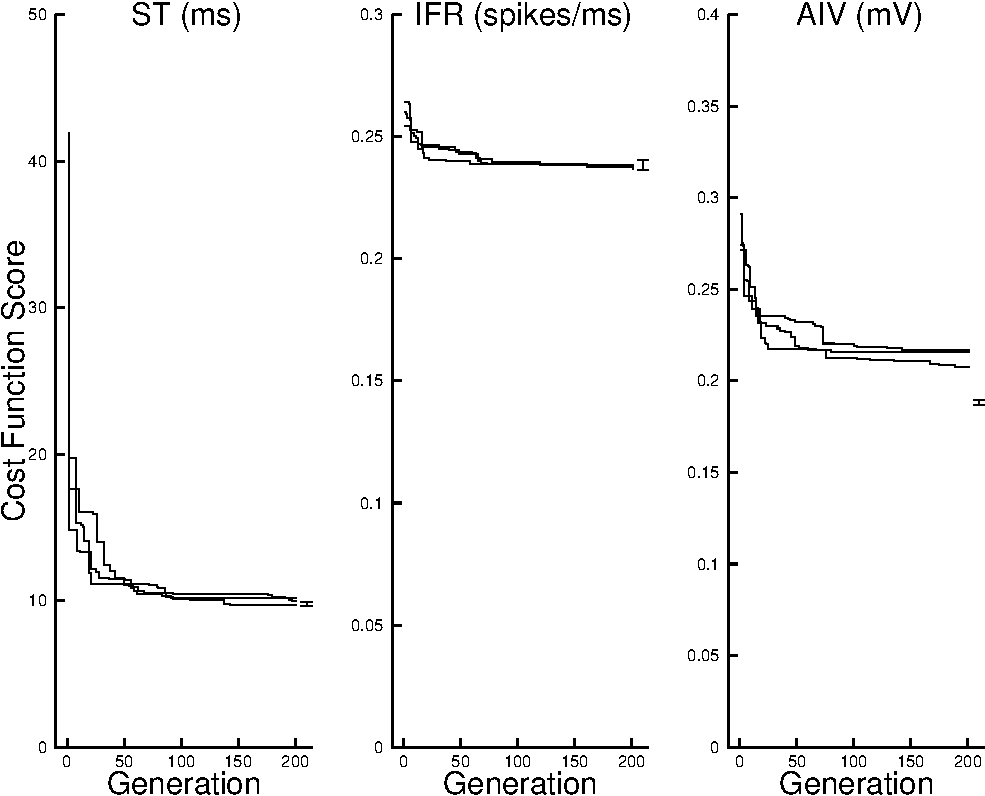
\includegraphics[width=\textwidth]{All25GAPerf-Stretch.eps}
  \caption{Performance of the GAs best performing genome in each
    generation is shown for each simulation. The mark to the right of
    each graph is the mean score and 95 percentile range of the target
    genome (error bars 2*sd).}\label{fig:R1}
\end{figure}

\medskip{}

For all three cost functions the best score obtained by the GA was considerably
above an error of zero. This does not imply poor performance by the GA, because
a perfect score of zero would require not only an exact match to the target
parameters, but also a precise match to the auditory nerve input spike trains
used in the target data. Experimentally the spike times of the auditory nerve
vary stochastically based on an instantaneous rate function for any given
stimulus. This stochasticity was incorporated into our model and led to non-zero
scores, even for the target network. The mean target score is shown by the error
bars on the right of each plot in Figure~\ref{fig:R1}.

\medskip{}

For the ST and IFR cost functions the best genome score was within the range of
scores found for the target network, indicating that the GA was able to find a
network that gave the same behaviour as the target network, as measured by the
cost function. For the AIV cost function, the best genome had a score that was
greater that the range of scores found for the target network, indicating a
discrepancy between the behaviour of the best network and that of the target, as
measured by the cost function.



\subsubsection{Cost Function Cross Comparison}

To facilitate the comparison of cost function performance, we used the best
genome from GA runs trained with one of the cost functions to evaluate the
remaining cost functions. This also allowed us to gauge how well that genome was
able to generalize to reproduce network behaviour as measured by the other cost
functions.


\begin{figure}[tb!]
  \centering
  \includegraphics[width=\textwidth]{boxplot25-sep-st.eps}\\
  \includegraphics[width=\textwidth]{boxplot25-sep-ifr.eps}\\
  \includegraphics[width=\textwidth]{boxplot25-sep-iv.eps}\\
  \caption{Cross comparison of best genomes generated using GA with 25
    repetitions, measured against the target, 1-step and 5-step
    parameter perturbation distributions.  The boxplots show the all
    three best genomes evaluated ten times for each cost function. 100
    evaluations of the target genomes were evaluated and 1000
    parameter perturbations were evaluated for the 1-step and 5-step
    distributions.}\label{fig:R2}
\end{figure}

\medskip{}

The results are shown in Figure~\ref{fig:R2A}, which compares the mean score
evaluated using the ST, IFR and AIV cost functions (Figures ~\ref{fig:R2A}A,
~\ref{fig:R2A}B and ~\ref{fig:R2A}C, respectively) for each of the three best genomes
obtained from GA runs trained with the different cost functions. In general, the
lowest scores were obtained when using the same cost function for evaluation as
was used for training of the best genome. 

\medskip{}

One AIV trained best genome generated ST scores around the target distribution,
however, the top graph shows that overall the IFR and AIV best genomes performed
relatively poorly when evaluated against the ST cost function.  The opposite
pattern was observed when the best genomes were evaluated with the IFR cost
function (middle plot), in which the ST best genomes performed poorly relative
to the IFR and AIV best genomes. All the best genomes gave similar scores for
the AIV cost function (bottom plot), but did not reach the target genome scores.

% the the ST trained genomes generalized
% well, in that the scores they obtained evaluating with the IFR and AIV cost
% function were close to the minimum score obtained across all genomes (i.e. the
% score obtained using the same cost function for the evaluation and training). In
% contrast, IFR and AIV trained genomes obtained relatively poor ST cost function
% scores compared with minimum score. They were, however, able to obtain near
% minimal scores with each other's cost function (i.e. the IFR trained genomes
% evaluated with the AIV cost function and vice versa).

% These results indicate that, in the current situation, training the GA using
% spike timing information gave a better general match to data than using
% repetition-averaged information involving spike rate or intracellular voltage.


% The results are given in
% Table~\ref{tab:Best25}, which lists the mean and standard deviation of cost
% function scores from evaluations with 100 stochastically different AN
% inputs. When evaluated with either the ST or the AIV cost functions, the best
% genome with the lowest score was the one trained using the cost function
% itself (indicated by a ``*" in each column); i.e. the ST trained genome gave
% lowest ST score and the AIV trained genome gave the lowest AIV score, amongst
% the different genomes. However when evaluated using the IFR cost function, the
% best genome trained with this cost function performed worse than the other two
% best genomes. Networks trained with ST and AIV cost functions generalized well
% when network behaviour was measured using the other two cost functions,
% whereas the network trained with the IFR cost function generalized relatively
% poorly.


% \begin{tabularx}{0.95\textwidth}{X|c|c}
%   Simulation                & MeanPE  & Score   \\\hline
%   stdyn diffAN sim1 min ga  & 22.1167 & 	10.1671 \\ 
%   stdyn diffAN sim2 min ga  & 31.6833 & 	10.0115 \\ 
%   stdyn diffAN sim3 min ga  & 12.7833 & 	9.67888 \\ \hline 
%   ifrga25 diffAN sim1 min ga& 22.2833 & 	0.238577 \\ 
%   ifrga25 diffAN sim2 min ga& 25.3167 & 	0.236389 \\ 
%   ifrga25 diffAN sim3 min ga& 28.5167 & 	0.23757 \\ \hline
%   ivga25 diffAN sim1 min ga & 26.2833 & 	0.216678 \\ 
%   ivga25 diffAN sim2 min ga &  25.45  & 0.207727 \\ 
%   ivga25 diffAN sim3 min ga & 29.3833 & 	0.21564 \\\hline
% \end{tabularx}

\clearpage

\begin{figure}[tb!]
  \centering
  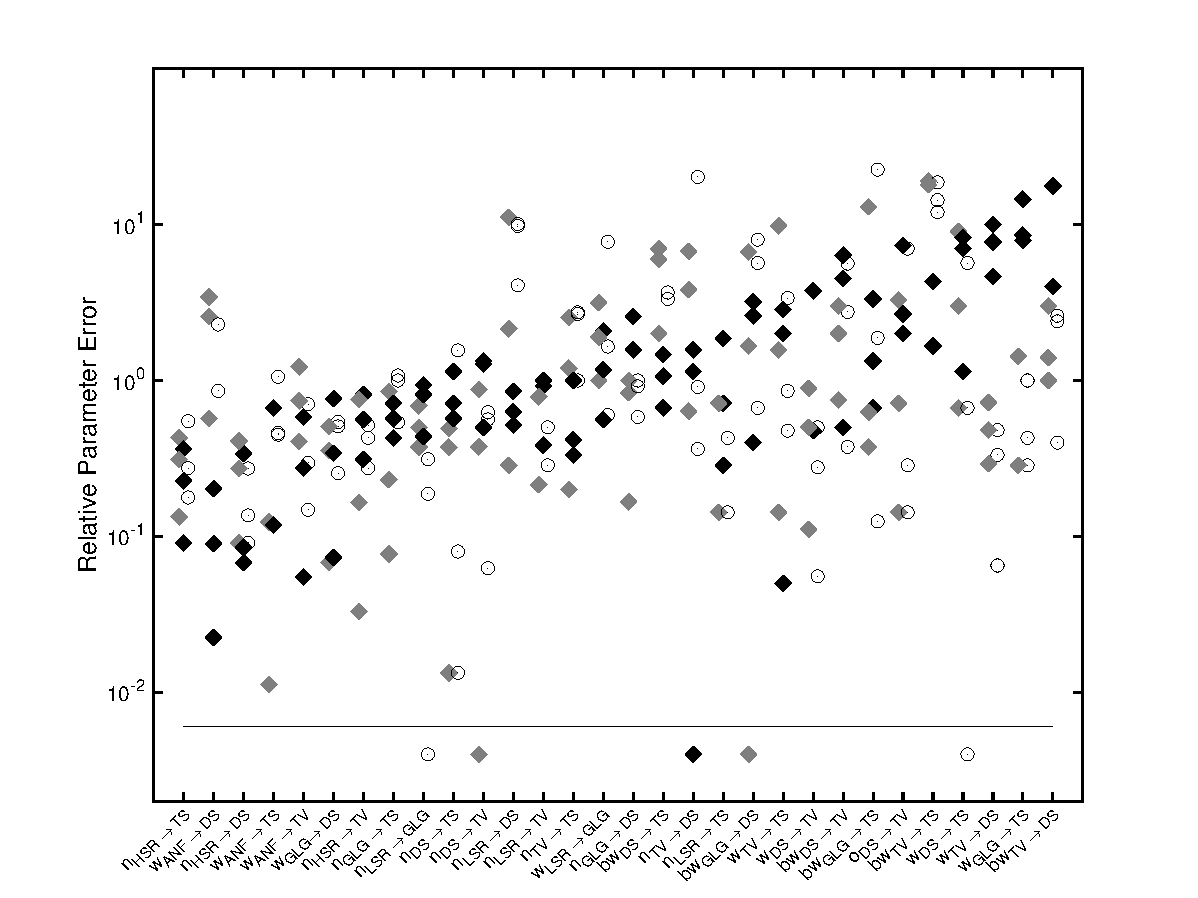
\includegraphics[width=\textwidth]{BestGenomesReRaw_CombinedLog}
  \caption{Parameter errors of the best genomes in 3 GA
    simulations for each cost function: ST (${\color{halfgray} \diamond }$), IFR (${\color{black} \diamond }$), and AIV (${\circ}$). Errors were normalised in terms
    of the target parameter values ( (target - bestgenome) / target )}\label{fig:R2b}
\end{figure}




\subsubsection{Match to Target Parameters}

A further way to evaluate GA performance is to compare the parameter values
between the best and target genomes by evaluating the relative error between
parameters (i.e. (target value - best value)/target value) . Individual relative
parameter errors are shown in Figure~\ref{fig:R2} for each of the best genomes
trained on a particular cost function. Parameters were ordered by increasing
mean relative error across all genomes.

\medskip{}

The plot shows a fairly similar level and pattern of performance across genomes
trained with the three different cost functions. Parameters were either
reasonably or poorly constrained independent of the cost function being used in
training. 

\medskip{}

In terms of parameter type, all bandwidth parameters were in the upper half of
genome errors whereas synapse number parameters were predominantly in the lower
half.  Weight parameters are spread over the whole range.


% {\it Still concerned that units are wrong. Percent error? Also v.hard compare
% cost functions. Plot on same figure? Looks like GA run variability is so large
% that nothing can be said about best cost function.}  The error has been
% measured in terms of the unit steps that were used to discretize the
% parameter. This is an arbitrary scale that relies on the designer of the GA
% choose a ``sensible" discretization scale for the parameters that
% 
% The lowest mean normalized parameter error was obtained by the AIV-trained
% best genome (0.207), followed by the ST-trained best genome (0.252) and the
% IFR-trained best genome (0.273). This order is consistent with performance of
% the different cost functions as evaluated by their cost function scores.

% In summary, the ST and AIV cost functions appear to perform better than the
% IFR cost function for GA optimization. This conclusion is supported by
% comparison of best genome scores relative to target scores, cost function
% cross comparisons and analysis of parameter errors.
%% Rearange order and comment on similarity.


% When the inputs were randomized and the training data (25~reps)
% remained the same, the GA populations' learning was considerably
% slower and the search space was more compact, Figure 6B. This meant
% that there was less difference between a good genome and a bad
% genome.  The best genome obtained by the IFR-25 cost function with
% different inputs had a score of 0.263~sp/ms and a mean parameter
% error of 0.273 (Figure~\ref{fig:8}D).
% 
% The performance of the best genome generated by the AIV-25
% cost function with different inputs was very accurate for inhibitory
% parameters (Figure~\ref{fig:8}G) presumably due to subthreshold
% information within the intracellular voltages.

\subsection{Parameter Sensitivity}

% Estimate of best performance possible given noisy input.
% 
% Comparison of ST, IFR and AIV.
% 
% Sensitivity - 1 step and 5-step.
% 
% Roughly equal sensitivity across cost functions.
% 
% The GA run using the ST cost
% function and different ANF inputs (Figure~\ref{fig:5}B) had a similar
% learning profile, but there was less variability in the 25--75
% percentile range in the later generations and the best genome score
% was 9.72~ms (Figure~\ref{fig:5}B).
% 
% 
% 
% When the inputs were
% randomized and the training data (25~reps) remained the same, the GA
% populations' learning was considerably slower and the search space was
% more compact, Figure 6B. This meant that there was less difference
% between a good genome and a bad genome.  The best genome obtained by
% the IFR-25 cost function with different inputs had a score of
% 0.263~sp/ms and a mean parameter error of 0.273
% (Figure~\ref{fig:8}D).
% 
% The AIV-25 and
% AIV-250 cost functions with different inputs scored, 0.208~and 0.188
% mV, respectively.  The mean parameter errors of the best genome for
% the AIV-25 cost function with identical inputs, the AIV-25 cost
% function with different inputs and the AIV-250 cost function with
% different inputs were, 0.258, 0.207 and 0.275, respectively (Figure
% 8F-H).

\subsubsection{Simultaneous Parameter Perturbation Analysis}

To better understand the relationship between cost function scores and the match
to target parameter values a parameter sensitivity analysis was performed. This
involved measuring the change in the cost function due to simultaneous
perturbations in all parameters.  Figure~\ref{fig:R3} shows the distribution of
cost function scores for different degrees of random simultaneous parameter
perturbation. Two populations of 1000 genomes were generated, one with parameter
values allowed to vary uniformly by 1 unit step either side of the target
(i.e. -1, 0 or 1 steps), and the second population was varied uniformly up to 5
unit steps.  In the 5 units step experiment, one parameter covers 11
combinations, including the target value.


\begin{figure}[tb!]
  \centering
  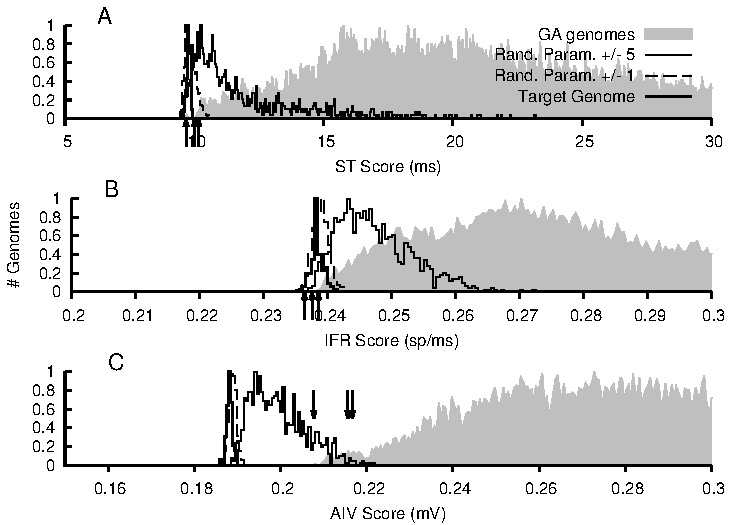
\includegraphics[width=\textwidth]{Histograms-Normalised.eps}  
  \caption{Histograms of simultaneous parameter perturbation of each cost
    function. The distribution of genomes in gray are all genomes evaluated by
    the GA that obtained the lowest score. The best scores of 3 GA simulations
    are pointed to by the arrows. The histograms show the distributions of 100
    target genome scores (thick line), 1000 genomes deviated by 1 unit step away
    from the target value (dashed line), and 1000 genomes deviated by 5 steps
    (thin line) from the target. The input spike generation and network
    connections for each parameter set (genome) were randomly generated for each
    evaluation.  All graphs are normalised to the peak value in each
    histogram.\label{fig:R3}}
\end{figure}

% In total the 5 units step experiment covers 9.72\% of
% the total parameter space and the 1 unit step experiment covers
% 2.65\%. {\bf What does this mean?? 11\% relative error = 1 step on average}

\medskip{}

In general, 1 unit step perturbations produced cost function scores both
slightly above and slightly below the range produced by the target network
(compare histograms in dashed versus bold lines, respectively). Five unit step
perturbations produced cost functions scores that were largely or wholly above
the target network range (compare histograms in thin solid versus bold lines,
respectively). This pattern was consistent across the three cost function
types. The shift of cost function scores to progressively higher values with
progressively larger perturbations is expected and desirable. It forms the basis
by which the GA performs optimization by comparing candidate genomes to the
target.

% The distribution of cost functions scores for the 5 unit step perturbation is
% less highly sensitivecost function in the vicinity of the target parameter
% valuesSeparated from target distribution for the IFR cost function than for
% either of the other cost functions. This is consistent with generally poorer
% performance of the IFR cost function.

\medskip{}

Best genomes scores from GA runs trained with either the ST or the IFR cost
function lay inside the range produced by the 1 unit step perturbation, whereas
best genomes scores from the GA runs trained with the AIV cost function were at
the upper limit of the range produced by 5 unit step perturbations. In fact,
Fig.~\ref{fig:R2} shows that all best genomes scored equally badly when
evaluated 100 times with the AIV cost function. Given this difference in AIV
cost function scores, it is worth noting again that pattern of change in cost
function distributions with perturbation size was fairly consistent across cost
function types. This suggests that the AIV cost function is equally well behaved
in the vicinity of the target compared to the other two cost functions. In this
case, the reason the best genomes trained with any cost function were unable to
attain a score in the target range (bottom plot of Figure~\ref{fig:R2}) was not
due to a poorly behaved cost function. % but further explanation is unknown


\medskip{}

It is, perhaps, surprising that the 1 unit step perturbations could produced a
network with lower cost function scores than the target network, albeit
marginally. This effect is the result of noise in the cost function, introduced
by the stochastic auditory nerve input: because the 1 unit step perturbations
involved 1000 separate instances of AN input, compared to only 100 instances for
the target, it was likely that a better match to the precise target AN input was
found amongst the former than the latter.  This effect is only expected to
become apparent for values of the cost function around the target score, where
systematic reduction of the cost function becomes increasingly marginal. This is
consistent with the observation that for larger, 5 unit step perturbations this
effect was much diminished or absent.



% When the target parameters were evaluated 100 times with different
% ANF input spikes the distribution of the ST cost function scores
% moved to 9.72~ms ($\pm$ 0.06~ms) (Figure~\ref{fig:9}B).  The 1-step
% distribution compressed around 9.79~ms for different inputs, As
% indicators of the GA's final performance, the best genomes produced
% by the GA of 8.45~ms (identical inputs) and 9.72~ms (different
% inputs) were very reasonable estimates.  The shape of the ST cost
% function distributions of 5 stp populations scores were very similar
% except for a positive shift with different inputs with means 10~ms
% and 11.8~ms, respectively.
% 
% Different ANF inputs had an adverse effect on the learning
% performance of the IFR-25 cost function, with the GA unable to find
% reasonable estimates near the global optimum
% (Figure~\ref{fig:10}B). The 1 step and 5 step scores were
% distributed around or close to the target scores showing a
% compression of the global optimum around 0.25~sp/ms
% (Figure~\ref{fig:10}B).
% 
% 
% Using different inputs, the target value of the AIV-25
% cost function is shifted to just above 0.2~mV, with the 1- and 5-step
% not far above. The best performing genomes in the GA were very close
% to the range of the 1-step and target genome scores (inset
% Figure~\ref{fig:11}B).




\subsection{Effects of Noise}

Noise from auditory nerve inputs could have a significant impact on
the GA optimization, with noise potentially preventing the GA from
attaining a good match to target. A simple way to reduce noise is to
use a larger sample of stochastic realisations of the AN input when
evaluating target and candidate genomes. This can reduce noise through
an averaging process, in the case of IFR and AIV cost functions or
through allowing more choice in matching spike trains in the ST cost
function. This would require using more stimulus repetitions when
collecting target data experimentally, and when simulating candidate
networks in the GA computationally. In this section we examine the
utility of this approach by comparing GA performance for 100 versus 25
stochastically distinct repetitions of the AN input for both target
and candidate genomes.

\medskip{}


\subsubsection{Increased Stimulus Presentations}


\begin{figure}[tb!]
  \centering
  % \figfont{A}\hspace{3.2in}\figfont{B}\\
  \includegraphics[width=\textwidth]{All100GAPerf-Log.eps}
  \caption{Performance of the GAs best performing genome run with 100
    repetitions in the fitness function. Each generation is shown for
    each simulation. The mark to the right of each graph is the mean
    score and error bars showing the range of 2 times standard
    deviation away from the mean target genome score.}\label{fig:R5}
\end{figure}

Figure \ref{Fig:R5} shows the evolution of best genome scores when 100
repetitions were used for the target and candidate genomes instead of
25 (as used in the results presented thus far). Overall the use of
increased repetitions of the stimulus resulted in reduced cost
function scores but did not result in better GA performance. This is
shown by the analysis given in Figure~\ref{fig:R6}.

\medskip{}

Similar to Fig~\ref{fig:R2}A, the figure compares scores across best genomes
trained with different cost function types (ST, IFR or AIV) and different
numbers of repetition (25 or 100) giving a total of six different best genomes
types: ST25, ST100, IFR25, IFR100, AIV25 and AIV100. The three different graphs
(Fig~\ref{fig:R2}A-C) correspond to evaluation of these best genomes using the
three different cost function types. The top of the lighter bars give the mean
score when 100 repetitions were used for evaluation, while the top of the
(appended) dark bars gives the mean score when only 25 repetitions were used
for evaluation.

\begin{figure}[tb!]
  \centering
  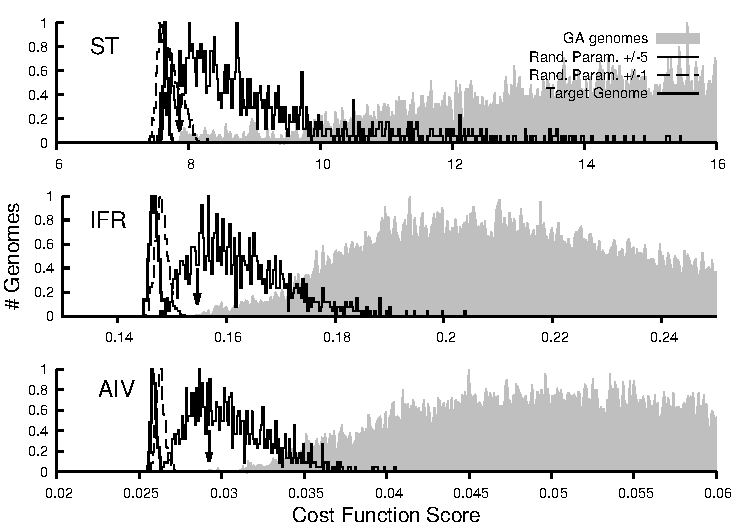
\includegraphics[width=\linewidth]{Histograms100-MaxNorm.eps}  
  \caption{Histograms of simultaneous parameter perturbation using 100
    repetitions. All graphs are similar to Fig.~\ref{fig:R4}.}
  % The
  % distribution of genomes evaluated during one GA are shown in gray
  % and the best scores of 3 simulation are pointed to by the
  % arrows. The histograms show the distributions of 100 target genome
  % scores (thick line), 1000 genomes deviated by 1 unit step away from
  % the target value (dashed line), and 1000 genomes deviated by 5 steps
  % (thin line) from the target. The input spike generation and network
  % connections for each parameter set (genome) were randomly generated
  % for each evaluation. 
  \label{fig:R6}
\end{figure}

\medskip{}

In all cases the use of 100 repetitions to evaluate the cost function
resulted in lower scores than when 25 repetitions were used (i.e. the
top of the dark bar lies above the top of the light bar). This did not
imply that genomes trained with 100 repetitions attained lower scores
than those trained with 25 repetitions, once the comparison was made
using the same cost function (i.e. same type, same number of
repetitions). In nearly all cases, scores for genomes trained using
different numbers of repetition (25 or 100), but the same type of cost
function (ST, IFR or AIV), obtained similar scores, regardless of the
details of the cost function used to evaluate them (i.e. ST25, ST100,
IFR25, IFR100, AIV25 and AIV100 cost functions). The exception was the
AIV100 trained genome when evaluated by the ST cost
function. % check statistical difference of AIV in ST

\medskip{}

This implies that, although the increased number of repetitions
reduced noise (and therefore cost function scores), this was not a
factor limiting GA performance.

\begin{figure}[tb!]
  \centering
  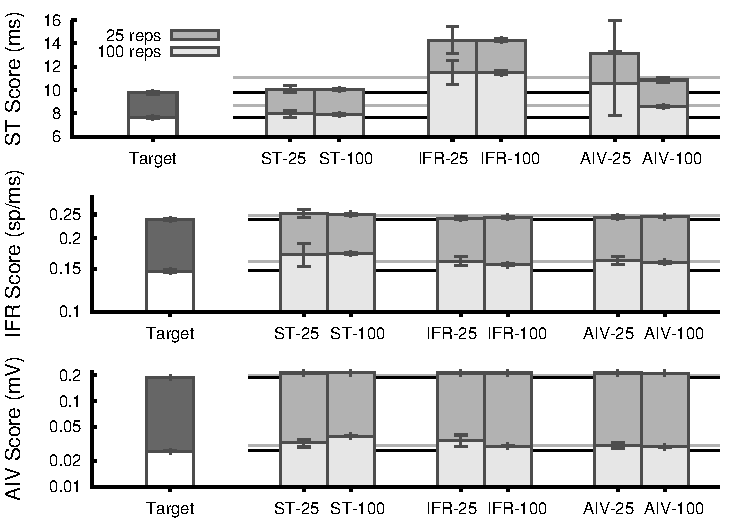
\includegraphics[width=\textwidth]{best25+100.eps}
  \caption{Comparison of Best genomes trained with different inputs
    using 100 or 25 repetitions.  Target genome was run 100 times and
    each GA best genomes were run 10 times. For reference, horizontal
    lines show the the median of the distribution of parameter
    perturbation for 1-step (dark line) and 5-steps (light
    line).}\label{fig:R7}
\end{figure}


\begin{table}[tb]
  \centering
  \begin{tabularx}{0.95\textwidth}{X|c|c|c}
    Cost Function &  PE$^*$ & Final GA Score & \\[0.5ex]\hline
    ST (ms)    & 1.977 &     7.86038    &  7.89 (0.04) \\
    IFR (spikes/ms)& 2.169 &    0.154698    & 0.1557 (0.00086) \\
    AIV (mV/ms)  & 2.325 &   0.0292369    & 0.0292 (0.000098)\\ \hline
  \end{tabularx}
  \caption{Best genomes obtained from GA's run with 100 repetitions. $*$ Mean relative parameter error }
  \label{tab:BestGenome100}
\end{table}

\begin{figure}[tb!]
  \centering
  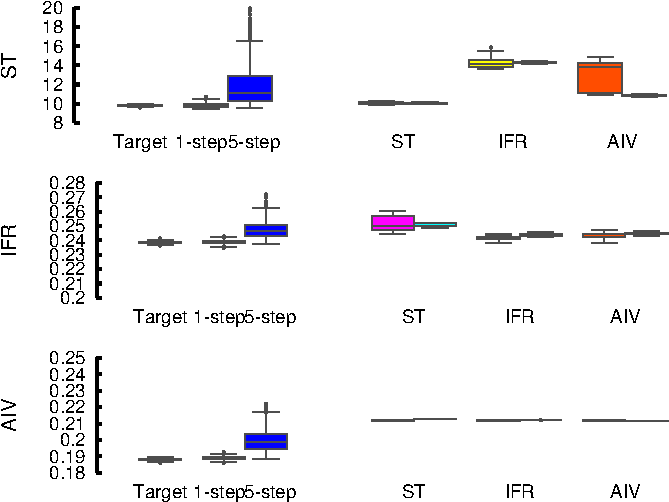
\includegraphics[width=\textwidth]{boxplot-100+25.eps}\\
  \caption{Cross comparison of best genomes generated using GA with
    100 repetitions, measured against the target, 1-step and 5-step
    parameter perturbation distributions.  The boxplots show the best
    genomes evaluated ten times for each cost
    function. }\label{fig:BestGenome100+25}
\end{figure}



% For comparison, also shown on these graphs are the best genome scores when
% only 25 repetitions were used, as well the accompanying histograms for the 1
% unit step perturbation analysis.
% 
% 
% {\it Perhaps present Figure showing target + best genome scores for ST, IFR
% and AIV trained as evaluated by each cost function} The 1 unit step
% perturbations scores for 100 repetitions are less than their counterparts for
% both 25 repetitions. This suggest that a substantial part of the cost function
% score, for 25 repetitions or ideal inputs, is attributable to noise. In the
% case of the ideal inputs, this noise is quenched in the form fixed random AN
% spike times and only becomes apparent when the number of synaptic connections
% in the network is perturbed from the target.
% 
%% Figure ? also shows that for the IFR cost function, the GA was able to make
%% use of this reduced noise to obtain a best genome with a score close to the
%% target score, but for the AIV cost function, the GA was not able to do
%% this. This is the reverse situation to when 25 repetitions were used for the
%% target.
% 
% Despite the reduction on cost function scores and noise did not help the GA
% find better parameter fits: surprisingly parameter errors were worse than with
% 25 repetitions.
%% 
%% The individual parameter sensitivity analysis showed a very similar pattern to
% the case with 25 repetitions: similar sets of parameters showed either bilateral
% sensitivity, unilateral sensitivity, insensitivity or contained opposing
% gradients. By contrast, the pattern of sensitivity for ideal inputs was quite
% different. This suggest that the greater sensitivity exhibited in the case of
% ideal inputs was due to the effects of quenched noise in the AN inputs.
% 
% Table ? shows a cross comparison of cost function scores for best genomes
% trained with either 25 or 250 repetitions for the target. It indicates that
% training with a 250 repetition target did not result in better performing best
% genomes. The best genome trained with 25 repetitions performed comparably to
% or better than the best genome trained with 250 repetitions, whether its
% performance was evaluated using a cost function with 25 of 250 repetitions.
% 
% In summary, the analysis indicates that although increased repetitions lead to
% lower cost function scores for the best genomes attained by the GAs, these
% best genomes were no better those trained with 25 repetition in terms of
% parameter errors or cross comparison of cost function scores. The reduction in
% cost function score is simply due to a reduction in noise, but appears to
% provide no benefit for the GA in terms of matching parameters to the target or
% reproducing the behaviour of the network.



% {\it Comment: There are two possible explanations for the increase in
% sensitivity when ideal input are used. The first is that the noise was masking
% an underlying trend or effect in the data, and that using ideal inputs
% eliminates this noises giving more sensitivity in the cost function to the
% underlying trend. The second is that the increased sensitivity for ideal input
% is a sensitivity to quenched noise in the input in the form of a specific set
% of spike times in the AN input. The former is a desirable property of the cost
% function, while the latter is not.
% 
% One way to differentiate between these possibilities is to increase the number
% of stimulus presentations. This can be used to reduce the noise by averaging
% and so better reveal the underlying effect. It is also a practical approach to
% overcoming the problem of input noise, since it can often be achieved
% experimentally.}



%%% Local Variables: 
%%% mode: latex
%%% TeX-master: "GAChapter"
%%% TeX-PDF-mode: nil
%%% End: 

\newpage
\include{ResultsIdeal}
\newpage
\section{Result 3: Individual Parameter Sensitivity near the Global Optimum}\label{sec:GA:IndividualSensA}


\subsection{Individual Parameter Perturbation Analysis}

To further understand how useful each cost function was in
constraining parameters, a sensitivity analysis on each individual
parameter is is crucial to understand the behaviour of individual
parameters close to the global optimum.  The sensitivity analysis of
the cost function is defined as calculating the learning gradients of
each parameter on either side of the target value. Parameter values
were stepped up and down independently, with the steps determined from
the gene resolution of the parameter in
Table~\ref{tab:GA:Genome}. Gradients were calculated using a
least-squares linear regression in MATLAB/GNU Octave and two-sided
t-tests were performed to determine whether each gradient was
significantly different from zero.  This was done for the identical
and the different ANF inputs, robustness was evaluated by comparing
the ratio of V-shaped to non-V-shaped cost function gradients for
different inputs.

\medskip{}

Representative examples are given in Figure \ref{Fig:R4}, which show
the dependence of the cost function on perturbation size when a parameter was
perturbed from its target value (and all other parameters had their target
value). A range of different behaviors is evident depending on the particular
combination of parameter and cost function. The ideal behaviour is shown in
Figure \ref{Fig:R4}A, which shows the target at a well defined local minimum in
the cost function, with significantly non-zero gradients bilaterally. Figure
\ref{Fig:R4}B is a sub-ideal case, with a significantly non-zero gradient
appearing only unilaterally, a zero gradient on the opposing side.  The
behaviour shown in Figure \ref{Fig:R4}C, in which the cost function is locally
flat, implies that the cost function is insensitive to this parameter in the
vicinity of the target and represents non-ideal behaviour. Finally, Figure
\ref{Fig:R4}D gives an example of a problematic cost function behaviour, in
which the minimum occurs at a value other than the target.\todo[inline]{Hamish: I am still not
happy we understand this well: Pruning of candidates with reduced spikes in
low rate regions of DS units}. These cases were classified variously as
bilaterally sensitive (Figure \ref{Fig:R4}A), unilaterally sensitive (Figure
\ref{Fig:R4}B), insensitive (Figure \ref{Fig:R4}C) or irregular(Figure
\ref{Fig:R4}D), respectively.

\todo[inline]{ Correlation between relative param error and gradient in Fig 5 to be discussed }

% The gradients of the cost function above and below the target value are plotted
% in Figure ? for each individual parameter and for the three different cost
% functions. {\bf order and comment on similarities. Also comment on correlation
% between parameter sensitivity and parameter error.}
% 
% A summary of these data are given in Table ?, which compares the cost
% function on basis of how many parameters showed sensitivity that was
% bilateral, unilateral or absent, or contained opposing gradients.

% I would be better to present these results in table comparing
% For different ANF
% inputs (Figure~\ref{fig:13}B), 11 parameters were bilaterally
% sensitive and 8 were unilaterally sensitive, while the ST cost
% function was completely insensitive to 6 parameters. Three parameters
% controlling the excitatory synaptic input to DS cells, 4, 5 and 6
% ($w_{{\rm ANF}\to {\rm DS}} $, $n_{{\rm HSR}\to {\rm DS}} $, $n_{{\rm
% LSR}\to {\rm DS}} $) had significant opposing gradients below the
% target, and the inhibitory input parameter 25 ($n_{{\rm TV}\to {\rm
% DS}} $) above the target suggesting a shifted optimum value.



 \begin{figure}[thp!]
   \centering
   \includegraphics[width=\textwidth]{./gfx/Example_SensAnalysis.eps}  
  \caption{Examples of ST cost function sensitivity analysis
    performed on individual parameters, with 10 unit step increments
    around the parameter's target value and all other target
    parameters retained. Multiple samples were taken at each point
    when different inputs were used. The linear regression line
    (solid) and bootstrapped 95\% confidence interval (dotted line)
    are shown. The slope was tested for significant difference to a
    zero gradient either side of the target value. (A) Parameter 3,
    $n_{{\rm HSR}\to {\rm TS}} $, was V-shaped for identical and
    different inputs. (B) Parameter 4, $w_{{\rm ANF}\to {\rm DS}} $,
    was V-shaped for identical inputs, but for different inputs the
    gradient below the target was significantly opposed to the
    correct direction. (C) Sensitivity around parameter 23, $s_{{\rm
        DS}\to {\rm TV}} $, was V-shaped for identical inputs but
    only one gradient was significant for different inputs. (D) The
    sensitivity of the ST cost function around parameter 29,
    $n_{{\rm GLG}\to {\rm DS}} $, produced the largest V-shaped
    gradients for identical and different inputs.}
  \label{fig:12}
\end{figure}



\begin{figure}[htb]
  \centering
  \caption{Parameter sensitivity gradient plots for the ST cost
    function with ideal input (A) and with different ANF input
    (B). Parameter gradients that are significantly different from
    zero (Student's t-test p $<$ 0.05) are shown with asterisk
    ($\ast$) and error bars that are the standard error of the
    slope. Gradients that are opposite to expected are shown in
    solid bars, with significant difference shown with a diamond
    ($\diamond$).}
  \label{fig:13}
\end{figure}



\begin{figure}[htb]
  \centering
  \caption{Parameter sensitivity gradient plots for the IFR cost
    function with the format similar to Figure~\ref{fig:13}. (A) The
    IFR-25 cost function with identical input. (B) The IFR-25 cost
    function with different ANF inputs. (C) The IFR-100 cost
    function with different ANF inputs.}
  \label{fig:14}
\end{figure}



\begin{figure}[htb]
  \centering
  \caption{Parameter sensitivity gradient plots for the AIV cost
    function with the format similar to Figure~\ref{fig:13}. A The
    AIV-25 cost function with identical input. (B) The AIV-25 cost
    function with different ANF inputs. (C) The AIV-100 cost
    function with different ANF inputs.}
  \label{fig:15}
\end{figure}




\subsubsection{Spike Timing}

\subsubsection{Instantaneous Firing Rate}

\subsubsection{Average Intracellular Voltage}


\subsubsection{Best Genome Match to Individual Parameter Sensitivity}

% 
% When the ANF input was slightly different from the ideal input, the optimum
% increases and the gradient of parameter 1, $w_{{\rm ANF}\to {\rm TS}}
% $, diminishes (Figure~\ref{fig:12}C). The spread of connections from
% DS cells to TV cells is wide (target value=8 channels), covering one
% third of the network (30 channels) so the non-linear jumps could be
% due to random selection of pre-synaptic cells or confounding effects
% of TV cells on TS and DS cells. With different inputs, parameter 23
% ($s_{{\rm DS}\to {\rm TV}} $) sensitivity of the ST cost function was
% robust below the target but is negative above the target although not
% significantly. Gradients that oppose the direction toward the target
% would reduce the effectiveness of optimization, especially
% gradient-decent methods.  For parameters with a target value close to
% the minimum range (parameters 17, 20, 26, and 27), the gradient below
% the target were not considered in the sensitivity analysis.
% 
% DS cells have very precise onset spikes and few spikes in the remainder
% of the stimulus.  If the weight and number of excitatory inputs were
% reduced, the spike timing difference would not be influence by (or
% inhibitory input increased), the onset spikes would still occur but
% the larger difference in the random positions the number of spikes in
% the sustained period of the stimulus would be reduced and the there
% would be some benefit to this change in the training data.
% 
% The sensitivity to inhibitory parameters of the
% IFR-25 cost function was not robust to changes in the ANF input
% (Figure~\ref{fig:14}B) since most gradients were flattened (not
% significant from zero gradient) or were unilaterally sensitive.  Seven
% inhibitory parameters had opposing gradients below the target, but
% only one was significant, 14 ($s_{{\rm DS}\to {\rm TS}} $). Parameter
% 10 had a significant reduction from identical inputs to different
% inputs, where it became completely insensitive.





%%% Local Variables: 
%%% mode: latex
%%% TeX-master: "GAChapter"
%%% TeX-PDF-mode: nil
%%% End: 

\newpage

%% * Discussion
%% ** General performance of GAs for optimising network parameters
%% ** Summary of cost functions
%% *** Spike Timing
%% *** Instantaneous Firing Rate
%% *** Average Intracellular Voltage
%% ** Effects of noise in BNN optimisation
%% *** Ideal or realistic neural input
%% *** Benefits of reducing noise by increased repetition
%% ** Sensitivity of parameters
%% ** Comparison with other studies
%% ** Other considerations for constraining BNNs
%% * Conclusion



\section{Discussion}\label{sec:GA:discussion}

\subsection{General performance of GAs for optimising network parameters}\label{sec:GA:general-perf}

We tested the ability of the GA to learn the network parameters of a
biophysically-based neural network (BNN) using three cost
functions. Figure~\ref{fig:GA:R1} showed the typical behaviour of GA populations,
with a convergence of the best genome toward the minimum value and the noisy
variation in the population of genome scores. GA's run with the ST and IFR cost
functions were able to consistently achieve convergence of the best genome to
very near the target score; the deviation was less than that due to a 1 unit
step perturbation of the target genome. For GA's run with the AIV cost function,
however, convergence of best genomes was inconsistent and did not reach the
target. Instead the AIV scores were limited to the upper tail of the
distribution obtained with 5 unit step parameter perturbations of the target
genome.

\smallskip{}

By increasing the number of repetitions in the GA evaluation, in
Figure~\ref{fig:GA:R5}, the cost function scores were reduced by the reduction in
noise. The GA performance did not lead to significantly improved match to the
target genome, with the exception of the AIV cost function.  The cost function
scores were significantly reduced for IFR and AIV cost functions but GA
performance did not lead to significantly improved match to the target genome.


\smallskip{}

keypoints:
* no basis for one CF better than another , 
* All performed similarly in most measures of comparison, X-comp and PE analysis
* X-comp: all best genomes performed similarly in IFR and AIV, but ST was better in it's won CF
* PE: similar trend/pattern similar PEvP in each given parameter (note significance of different parameter types - orders of 2 or 3 between spread/numberand weight parameters)

* noteworthy: ST Xcomp: expected result AIV Xcmomp: ST does not
perform poorly on AIV given different characteristics of CF,
i.e. spike timing does not provide information about
sub-threshold membrane potential, a relevant factor in the AIV
CF.  But this is good because, ST can be obtained in extra
cellular recordings more easily in vivo and can be obtained on a larger
number of simultaneous units than intracellular recordings.


*       IFR consistently off in ST and AIV
AIV CF also limited  ST and IFR best genomes to same limit as AV best genome 



\subsection{Summary of cost functions}\label{sec:GA:summ-cost-funct}

This section gives an overview of the cost functions' advantages, disadvantages,
and relevance to optimizing BNNs. The following summary of the cost functions
will highlight and compare the results by focusing on three main performance
measures.  Measure 1 indicates whether the best genome obtained a \textit{poor},
\textit{good}, or \textit{very-good} score. Very good scores are below the mean
of the 1-step deviation population, poor scores are above the mean of the 5-step
deviation population, and good scores are in between.  %Measure
% 2 indicates the robust sensitivity of the cost function and is the
% ratio of significant V-shaped sensitivity gradients with different AN
% inputs against other less sensitive parameters (i.e any shape that is
% significantly non-V-shaped or other V-shapes that are not
% significant). The gradients below the target value of parameters 17,
% 20, 26, and 27 were ignored, as explained in section
% 3.3~\textit{Individual Parameter Sensitivity near the Global Optimum}.
Measure 2 gives the relative geometric distance between the target
parameter set and the target genome's parameters.

\subsubsection{Spike timing}\label{sec:GA:spike-timing-summ}

The results of the ST cost function show that it can be successfully used for
optimising BNNs.  For Measure 1, the results were very-good for the best genome
with different inputs as it scored below the mean of target genome scores. It
also achieved a good score when evaluated with the other cost functions.  For
Measure 2, the mean geometric distance between the ST best genome and the target
was 0.252, the second best next to the AIV-25 cost function for GA simulations
run with different AN inputs.

\smallskip{}

A major benefit in using spike times in optimisation of real networks is their
ease of collection \textit{in vivo}. Data from populations of neurons can be
obtained by extracellular single- or multi-unit recordings.  By sampling over
all cells multiple times, this method provides a good estimate of the temporal
information contained in the neural responses, enabling reasonable parameter
optimisation and good robustness to noise.  The key disadvantage associated with
spike train comparisons is the increased computational time associated with the
evaluation of the cost function score.  For $R=25$ repetitions, the ST cost
function took just as long to run as the CN network simulation time
(approximately 90 seconds in a single 2GHz CPU) depending on the level of
activity. Increasing the number of repetitions scaled the computation time by
$R^2$ due to the cross comparison of available spike trains in the training data
to find the minimum error.

\smallskip{}

Noise was minimised by the comparison procedure that found the minimum score
among 25 spike trains in the training data. Any additional data from more
repetitions or more neurons may be beneficial for the robustness to noise, but a
combination with another source of data, for example AIV waveforms, would be
more suitable. The dynamic programming algorithm in the ST cost function is
similar to the temporal difference method of \citet{VictorGoldbergEtAl:2007},
except that specific penalties were not applied to insertions and deletions of
spikes.

% The synaptic parameters have a strong influence on the timing of spikes in
% post-synaptic neurons, contributing to changes in the cost function score when
% the parameters are moved further away from the target, and provide a
% well-defined global optimum. Even though the number of individual parameters
% with significant learning gradients was reduced for the ST cost function with
% different inputs and there were four parameters with significant opposing
% gradients (Figure 13B), the cost function still produced a distinctive optimum
% (Figure 9B) and tqhe GA was able to find genomes close to the global optimum.

\subsubsection{Instantaneous Firing Rate }\label{sec:GA:inst-firing-rate-summ}

\todo[inline]{Hamish noted that this para was not applicable} When considering the 25
repetition IFR cost function's performance, Measure 1 for the best genome
obtained with different inputs was poor for all cost functions. When the number
of repetitions in the training data was increased by a factor of 4 (the IFR-100
cost function), there was a reduction in the value of all cost function scores
(Figure~\ref{fig:GA:R6}B) and the performance of the best genomes was good (Figure
\ref{fig:GA:R7}). However, the performance of both the IFR-25 and IFR-100 best
genomes when measured using the other cost functions was poor, this suggests
that the networks constrained by the IFR cost functions were unable to
accurately reproduce the behaviour of networks in terms of spike-times or
intracellular voltage. %The individual parameter sensitivity measure,
% Measure 2, gave a ratio of 7:23~and 9:21~for the IFR-25 and IFR-250
% cost functions, respectively (Figure~\ref{fig:GA:14}B,C), demonstrating a
% high susceptibility to input noise. Constraint of inhibitory
% connections (parameters 12-30) in the IFR best genomes
% (Figure~\ref{fig:GA:8}D,E) was very poor, resulting from the flat and
% insignificant cost function gradients near the global optimum (Figure
% 14B,C).
For Measure 2, the results of the IFR-25 and IFR-100 best genomes found using
different inputs show large mean parameter errors of 0.273~and 0.297,
respectively (Figure~\ref{fig:GA:8}D-E).

\smallskip{}

Grouping spike trains into time bins is a very fast procedure aimed at reducing
the trial-to-trial variability in single spike trains by generating an estimate
of the average instantaneous firing rate of neurons. The temporal resolution of
the IFR cost function is dependent on the width of the PSTH bins but it looses
information about the timing between spikes.  The representation of precise
onset spikes in DS and TS cells would benefit from a narrow bin width, but for
the majority of spikes in the network, the fine timing is not as important
during a noisy stimulus.  For the frozen notch noise, spatio-temporal peaks in
neural activity occur across the network and require enhanced temporal precision
in the IFR cost function, as shown in Figure~\ref{fig:GA:Costfunctions}.

\smallskip{}

To improve the representation of firing-rate information, we must take into
consideration the width of the bins in a PSTH and their relationship to the
stochastic output of neurons.  It is desirable to have fine temporal resolution,
but the results of the IFR cost function show that the small bins are dominated
by noise, especially in low-firing units and in onset units apart from the first
spikes. A solution to this problem in future experiments would be to use
equi-probable bins in linear or log form \cite{BhumbraInyushkinEtAl:2004}.  This would improve the
performance of the IFR cost function by improving the sensitivity to changes in
parameters of the network.

\subsubsection{Average Intracellular Voltage}\label{sec:GA:aver-intr-volt-summ}

For Measure 1, the best genome constrained by the AIV-25 cost function was very
good when evaluated using all cost functions (Table~\ref{tab:GA:5}) except for the
ST cost function for which it was good. The best genome trained using the
AIV-100 cost function was also very good for the ST, IFR-100, and AIV-25 cost
functions, and good for the IFR-25 and AIV-100 cost
functions.  % For Measure 2, the sensitivity
% ratios of individual parameters using different inputs were 13:17 and
% 9:21 for the AIV-25 and AIV-250 cost functions, respectively
% (Figure~\ref{fig:GA:15}B,C).  This demonstrates that the AIV-25 cost
% function has greater robustness to noise than the AIV-250 and the IFR
% cost functions, and similar performance to the ST cost function.
For Measure 2, the parameter error of 0.207~for the AIV-25 best genome was the
best for all GA simulations that were run with different inputs in this study,
while the AIV-100 best genome was further from the target genome with an error
of 0.275 (Figure~\ref{fig:GA:8}G,H).

\smallskip{}

The average IV waveform over several repetitions aimed to reduce the effect of
trial-to-trial error and filter out APs.  Similar to the point-to-point method
comparison in the IFR cost function, increasing the number of repetitions
smoothed out the training data in the AIV-100 cost function scores and reduced
the scores for parameters close to the target (1-step and 5-step) reduced to the
level of the ideal scores (Figure~\ref{fig:GA:11}A,C).

\smallskip{}

It was thought that for a BNN model the average IV waveform will provide
additional information about the sub-threshold behavior of neurons in the
network, which is not available in the ST and IFR cost functions.  Intracellular
voltage data has been used in constraining the membrane conductances of
multi-compartmental single-neuron models \cite{Le_Masson:2000,KerenPeledEtAl:2005}.
These methods are not always effective in single simulations unless combined
with other cost functions, such as inter-spike intervals
\citep{KerenPeledEtAl:2005}. Phase-plane analysis of IV data was very effective
in optimizing membrane parameters \citep{VanDeEtAl:2008,KerenPeledEtAl:2005} but would not
be suitable to a BNN due to variation in the synaptic input and the loss of
temporal information.  It is not currently possible to obtain simultaneous IV
recordings from more than two neurons let alone a whole nucleus, but limited IV
data could be used in conjunction with other cost functions to constrain BNN
models.

\subsection{Benefits of reducing noise}\label{sec:GA:benef-reduc-noise}

\smallskip{} 

\todo[inline]{ Must fill this out before sending back to hamish}
*No real differences in eventual performance
  despite reduction in score

** Lower cost function scores for all CFs

** Fig R7 Xcomp shows GA best genomes run with 25
    performed approx the same as GA's run with 100
** only clear exception being AIV 100 significantly better in ST CF

** noteworthy AIV limitations from 25 reps were removed
  in 100 reps, with the best genome's score were closer to the target
  (less than mean of 5 unit step perturbation).

\smallskip{}

One of the big problems in optimizing BNNs is noise.  The various sources of
noise arise in the stochastic nature in neural transmission and connectivity
and in the algorithm chosen by the cost functions. Afferent input connections
and intrinsic connections within the microcircuit are defined by organised but
random connectivity.  Small perturbations in the parameters controlling the
number of inputs will change the selection of pre- and post-synaptic cells in
the construction of the network.  The smoothing of PSTH and IV also produces
inherent errors in the training data for parameters near the target
parameters, some of which perform better.  The main effect of noise in
optimization is over-fitting to the noise, resulting in a best genome scores
that are better than the target genome's distribution scores.  The GA run with
ST cost function and different inputs produced a score better than the mean
target with only one sample, when sampled multiple times the mean score was
also below the mean target scores but not statistically significantly.  In all
cost functions, the flattening of the cost function search spaces around the
target parameters contributed to an overlap between the 1-step population and
the distribution of the target genome.

\subsection{Sensitivity analysis of individual parameters}

This section gives an overview of the cost functions' advantages,
disadvantages, and relevance to optimizing BNNs with regard to
parameter sensitivity.  A measure to indicate the robust sensitivity
of the cost function is the ratio of significant V-shaped sensitivity
gradients with different AN inputs against other less sensitive
parameters (i.e any shape that is significantly non-V-shaped or other
V-shapes that are not significant). The gradients below the target
value of parameters 17, 20, 26, and 27 were ignored, as explained in
section~\ref{sec:GA:IndividualSensA}.

\smallskip{}

The sensitivity measure is mixed for the ST cost function with a ratio
of 13:17 for V-shaped and non-V-shaped parameter gradients and 7 other
parameters were significant on only one side. Also, there were four
significant gradients that were in the direction away from the target
(Figure~\ref{fig:GA:13}B).

\smallskip{}

The IFR-25 cost function sensitivity measure gave a ratio of 7:23
(Figure~\ref{fig:GA:14}), demonstrating a high susceptibility to input
noise. Constraint of inhibitory connections (parameters 12-30) in the
IFR best genomes (Figure~\ref{fig:GA:8}) was very poor, resulting from
the flat and insignificant cost function gradients near the global
optimum (Figure ~\ref{fig:GA:14}).

\smallskip{}

The sensitivity ratios for the AIV-25 cost function were 13:17
(Figure~\ref{fig:GA:15}B).  This demonstrates that the AIV-25 cost
function has greater robustness to noise than the IFR cost function,
and similar performance to the ST cost function.

\smallskip{}

In general, parameters 3, 9, 11, and 29 (corresponding to \nHSRTS,
\nHSRTV,\nLSRGLG, and \nGLGDS, respectively) were more robust to the
variability of input spike times in each of the cost functions.  The
number of connections between a cell type and one post-synaptic cell
provides a greater influence on the synaptic strength between cells
than the synaptic weight (despite being uniform across all synapses in
this connection type). This can have a compounding effect on any
connected cell group that receive input from the pre-synaptic cell
group.


\subsection{Comparison with other studies}\label{sec:GA:comp-with-other}


\todo[inline]{GA could not have done an better than any other optimisation techniques.
Evolutionary vs Grad decent studies?  Consistency, efficiency for BNNs.}

\smallskip{}

\todo[inline]{*Studies with  other cost functions - do they get close to target? ISI CF studies?
Are there any studies showing ST and IFR/AIV? any comparisons?}

\subsection{Other considerations for constraining BNNs}\label{sec:GA:other-considerations}


In this chapter limiting the number of parameters used to define the connectivity
of a BNN was critical for a practical method of optimization. Simplifying the
synaptic strength between two cell types to uniform weight and number
significantly reduced the number of parameters required for optimization, but
uniformity is unlikely for the real network weights.  A Gaussian weight
distribution is common among network models and would only add one parameter per
connection (i.e.\ standard deviation with the existing uniform mean parameter).
Optimizing conduction- and synaptic-delay is not covered in this paper, but
could add to further realism in BNN optimization.

\smallskip{}

A final issue that should be considered for modelling and optimizing BNN models
is computational efficiency. In this paper, the CN stellate network consisted of
240 HH-like cells, simulated in NEURON and took approximately 90 seconds to run
a 80~ms stimulus on a 1.8 GHz CPU (32-bit Itanium, SGI Altix).  Evaluations the
AIV and IFR cost functions were a minor fraction of the total computational
time, being less than 3 seconds per network. The ST cost function was at a
considerable disadvantage because its evaluation took approximately 90 seconds,
which is similar to the simulation time. This could be improved because the
method for calculating the dynamic programming spike time distance was
sub-optimal.  On the 64-CPU SGI Altix, the amount of time required to run the GA
for 201 generations of 100 genomes took approximately 8 hours (a maximum of 40
CPUs were used at any point.  These computational loads are feasible in modern
systems and will enhance the development of more realistic BNN models.


\section{Conclusion}\label{sec:GA:conclusion}

The methods for generating experimentally relevant data are an important factor
when constraining a BNN model. In an ideal network model, where we can reproduce
the exact inputs to the network, as used in generating the training data, it
brings into question the validity of the training data to reproduce real
experiments.  Training data from an existing model, with target parameters
chosen randomly as performed in this paper, does not give us a representation of
a real network, but the development of methods for constraining new models is an
important step for generating microcircuits and larger networks.

\smallskip{}

In this chapter, we have shown that the GA is an adequate method for parameter
optimization and that the ST and AIV cost functions are comparably good methods
for constraining BNNs. Further development is needed to enhance the robustness
of the cost function methods to input noise, especially for sensitivity and
robustness of inhibitory connections in the CN stellate network.
\todo[inline]{Last section you need to improve when you are done}


%%% Local Variables: 
%%% mode: latex
%%% TeX-master: "GAChapter"
%%% TeX-PDF-mode: nil
%%% End: 




%%%%%%%%%%%%%%%%%%%%%%%%%%%%%%%%%%%%%%%%%%%%%%%%%%%%%% 
%\begin{appendicies}
\appendix

\section{GAChapter Appendix}\label{sec:GA:chapter-5-appendix}

\subsection{Extra Data}

\begin{table}[htp]
  \centering
  \caption{Comparison of best genomes using {GA} with
    identical inputs. * Indicates the best cost function score from
    each {GA}}\label{tab:GA:4}
  % \begin{tabular}{p{1.5in}*{3}{c}} \hline
  \begin{tabular}{lccc}
\toprule
                   &       ST       &     IFR-25      & IV-25 \\
\midrule
  Target Genome    &       0        &        0        & 0 \\ %\hline
1-step Population  &  7.32 (0.89)   &  0.184 (0.011)  & 0.134 (0.009)\\ %\hline
5-step Population  &   10.0 (3.0)   &  0.209 (0.012)  & 0.165 (0.014) \\ %\hline
 ST Best Genome    & \textbf{8.45}* &      0.202      & 0.183 \\ %\hline
IFR 25 Best Genome  &      12.2      & \textbf{0.195}* & 0.180 \\ %\hline
%IFR 250 Best Genome &      10.8      &      0.207      & 0.178 \\ %\hline
IV 25 Best Genome  &      9.58      &      0.202      & \textbf{0.158}* \\ %\hline
%IV 250 Best Genome  &      9.52      &      0.207      & 0.159 \\
\bottomrule
\end{tabular}
\end{table}


\begin{table}[tbh]
  \centering
  \caption{Cross comparison of best genomes from GA simulations using different ANF inputs.}
  \label{tab:GA:XComp}
%  \input{src/best_genomes_25.tex}
\end{table}




\begin{table}[tp]
 \centering
 \caption{Comparison of Best genomes trained with different
   inputs.  Target genome and each {GA} best genomes were run 100
   times. One thousand genomes were run with different inputs in the 1
   step and 5 step parameter variation population.}\label{tab:GA:5}
 % \begin{tabular}{|p{1.1in}|p{0.3in}|p{0.3in}|p{0.3in}|p{0.4in}|p{0.3in}|p{0.4in}|p{0.3in}|p{0.4in}|p{0.3in}|p{0.4in}|}\hline
% \begin{tabular}{p{1.0in}*{10}{c}}
%\hline
%                        & \multicolumn{2}{c}{ST}  & \multicolumn{2}{c}{IFR-25} & \multicolumn{2}{c}{IFR-100} & \multicolumn{2}{c}{AIV-25} & \multicolumn{2}{c}{AIV-100} \\
% \hline
%     Target Genome       &      9.72      & (0.06) &     0.237      &  (0.001)  &     0.157      &  (0.001)   &      0.206      & (9e-4) & 0.128 & (0.001) \\ %\hline
%   1-step Population     &      9.79      & (0.23) &     0.237      &  (0.001)  &     0.158      &  (0.001)   &      0.207      & (0.001) & 0.129 & (0.002) \\ %\hline
%   5-step Population     &      11.8      & (2.6)  &     0.246      &  (0.006)  &     0.171      &  (0.009)   &      0.219      & (0.008) & 0.149 & (0.01) \\ %\hline
%   ST {\GA} Best Genome     & \textbf{9.63}* & (0.06) &     0.242      &  (0.001)  &     0.164      &   (9e-4)   &      0.214      & (9e-4) & 0.140 & (9e-4) \\ %\hline
% IFR 25 {\GA} Best    Genome &      15.0      & (0.2)  & \textbf{0.247} &  (0.001)  &     0.171      &  (0.001)   &      0.237      & (0.001) & 0.173 & (0.001) \\ %\hline
% IFR 250 {\GA} Best Genome  &      16.8      & (0.4)  &     0.243      &  (9e-4)   & \textbf{0.165} &  (0.001)   &      0.244      & (9e-4) & 0.183 & (0.001) \\ %\hline
%  IV 25 {\GA} Best Genome   &      11.3      & (0.1)  &     0.238*     &  (0.001)  &     0.159*     &   (9e-4)   & \textbf{0.211*} & (9e-4) & 0.136* & (8e-4) \\    % \hline
% IV 250 {\GA} Best Genome   &      10.4      & (0.1)  &      0.24      &  (0.001)  &     0.161      &  (0.001)   &      0.213      & (9e-4) & \textbf{0.138} & (0.001) \\
% \hline
% \end{tabular}

%  \input{src/best_genomes_100.tex}
 \end{table}


\subsection{C++ Code: \textsf{ganeuron}}\label{sec:GA:cpp-code}

\subsection{NEURON Code: \textsf{opt4}}\label{sec:GA:neuron-code}



\clearpage


%%% Local Variables: 
%%% mode: latex
%%% TeX-master: "GAChapter"
%%% TeX-PDF-mode: nil
%%% End: 

%\end{appendicies}

%%%%%%%%%%%%%%%%%%%%%%%%%%%%%%%%%%%%%%%%%%%%%%%%%%%%%% 
 \bibliographystyle{abbrvnat}%plainnat}%bmc_article} % Style BST file
 \bibliography{../MyBib}



\end{document}

%%% Local Variables:
%%% mode: latex
%%% mode: tex-fold
%%% TeX-PDF-mode: nil
%%% TeX-master t
%%% End: 
